\documentclass[11pt,a4paper,oneside]{article}

%% =========================== Global flags ============================== %%

% !TEX root = ./doptrack.budget.tex

% ===== Global options =====

% % uncomment this to turn on draft features
% \let\draft

% uncomment this to include the list of symbols/acronyms
\let\IncludeAcronymList

% % uncomment this to use natbib
% \let\UseNatBib


% ===== Acronyms options =====

% comment to remove the definition of all acronyms (i.e. any use of \ac{acronym} will produce an error)
% comment this in case no acronym is used, otherwise latex complains that "Something's wrong--perhaps a missing \item"
\let\UseAcronyms

% % comment to remove citations from some acronyms
% \let\UseCitationsInAcronyms

% % comment to remove section references from some acronyms (need to have defined a number of labels, do 'grep acroref acronyms.tex' to see which)
% \let\UseReferencesInAcronyms


% ===== Symbols options =====

% comment to remove the definition of all symbols (i.e. any use of \ac{symbol} will produce an error)
% comment this in case no acronym is used, otherwise latex complains that "Something's wrong--perhaps a missing \item"
% \let\UseSymbols

% % uncomment this to add explanatory text to the list of symbols
% \let\IncludeSymbolsText

% % uncomment to have section/chapter definitions in the list of symbols
% \let\IncludeSymbolsSections

% % uncomment to see all symbols, including plurals and $_i$ forms (useful only in debug)
% \let\IncludeListWithAllSymbolForms

%% ========================  packages  ========================== %%

% !TEX root = ./tracking.groundstation.budget.tex

%% =========================== Packages used ============================== %%

% Ex­tended UTF-8 in­put en­cod­ing sup­port
\usepackage{ucs}                            % http://www.ctan.org/pkg/ucs

% Ac­cept dif­fer­ent in­put en­cod­ings
\usepackage[utf8x]{inputenc}                % http://www.ctan.org/pkg/inputenc

% To use English hyphenation
\usepackage[british]{babel}                 % http://www.ctan.org/pkg/babel

% Flex­i­ble bib­li­og­ra­phy sup­port
\ifdefined\UseNatBib
  \usepackage[round,sort]{natbib}           % http://www.ctan.org/pkg/natbib
\fi
% Ver­ba­tim with URL-sen­si­tive line breaks
\usepackage{url}                            % http://www.ctan.org/pkg/url

% mathematical facilities
\usepackage{amsmath}                        % http://www.ctan.org/pkg/amsmath

% typeset text fragments in mathematics
\usepackage{amstext}                        % http://www.ctan.org/pkg/amstext

% LATEX support file to use the WASY2 fonts
\usepackage{wasysym}                        % http://www.ctan.org/pkg/wasysym

% Mathematical fonts to fit with particular text fonts
\usepackage[utopia]{mathdesign}             % http://www.ctan.org/pkg/mathdesign

% Intermix single and multiple columns in tables
\usepackage{multicol}                       % http://www.ctan.org/pkg/multicol

% Create tabular cells spanning multiple rows
\usepackage{multirow}                       % http://www.ctan.org/pkg/multirow

% Scale Computer Modern fonts properly
\usepackage{type1cm}                        % http://www.ctan.org/pkg/type1cm

% needed to reset paragraph counters every new section
\usepackage{chngcntr}                       % http://www.ctan.org/pkg/chngcntr

% needed to display bold-face greek symbols
\usepackage{bm}                             % http://www.ctan.org/pkg/bm

% allows for figures filenames to contain dots
\usepackage[multidot]{grffile}              % http://www.ctan.org/pkg/grffile

% pretty sub-figures
\usepackage{subfig}                         % http://www.ctan.org/pkg/subfig
\captionsetup[subfigure]{margin=10pt,justification=centerlast}
% acronyms handling:
% define: \acrodef{label}[acronym]{written out form}
% normal usage: \ac{label}
% written out form with acronym in parentheses: \acf{label}
% acronym form: \acs{label}
% written out form without following acronym: \acl{label}
% starred forms does not mark the acronym as used: : \acp*,\acfp*,...
% plural form of acronym by adding an s: \acps,\acfps,\acsps,\aclps
\ifdefined\IncludeAcronymList
  \usepackage[printonlyused]{acronym}       % http://www.ctan.org/pkg/acronym
\else
  \usepackage[nolist,nohyperlinks]{acronym}
\fi

% make floats stick to the current section
\usepackage[section,verbose]{placeins}      % http://www.ctan.org/pkg/placeins

% strike-through, underlines, etc
\usepackage[normalem]{ulem}                 % http://www.ctan.org/pkg/ulem

% provides \sfrac (slanted fractions, the same as $^{num}/_{denom}$ but prettier)
% \usepackage{xfrac}                          % http://www.ctan.org/pkg/xfrac

% allows for the same functionality of pageref (otherwise broken) using \getpagerefnumber{key}
\usepackage{refcount}                       % http://www.ctan.org/pkg/refcount


% allows m{<widht>} specifications in table columns that are vertically centred.
\usepackage{array}                          % http://www.ctan.org/pkg/array

% prevents floats from appearing after the next section and where \FloatBarrier is manually placed
\usepackage[section]{placeins}              % http://www.ctan.org/pkg/placeins

% diagrams!
\usepackage{tikz}                           % https://www.sharelatex.com/learn/TikZ_package
\usetikzlibrary{shapes,arrows}

\usepackage{etoolbox}                       % http://www.ctan.org/pkg/etoolbox

% A multi-page tables package
\usepackage{supertabular}                   % http://www.ctan.org/pkg/supertabular

% Provides the \ifpdf conditional
\usepackage{ifpdf}                          % http://www.ctan.org/pkg/ifpdf

% \usepackage{calculator}

% package selection according to pdftex/dvips methods
\ifpdf
  %Subliminal refinements towards typographical perfection
  \usepackage{microtype}                    % http://www.ctan.org/pkg/microtype

  % Enhanced support for graphics
  % \usepackage[pdftex]{graphicx}           % http://www.ctan.org/pkg/graphicx

  % color in text (conflicts with graphicx)
  \usepackage{color}                        % http://www.ctan.org/pkg/color

  % color in the tables
  \usepackage{colortbl}                     % http://www.ctan.org/pkg/colortbl
  \ifdefined\draft
    % Extensive support for hypertext in LATEX
    \usepackage[pdftex,unicode,
                draft=false,
                pdffitwindow=true,
                pdfpagemode=UseThumbs,
                pdfpagelabels,
                breaklinks=true,
                colorlinks=true,
                linkcolor=black,
                citecolor=black,
                filecolor=black,
                urlcolor=black] {hyperref}  % http://www.ctan.org/pkg/hyperref
  \else
    \usepackage[pdftex,unicode,
                final=true,
                pdffitwindow=true,
                pdfpagemode=UseThumbs,
                pdfpagelabels,
                breaklinks=true,
                colorlinks=true,
                linkcolor=black,
                citecolor=black,
                filecolor=black,
                urlcolor=black] {hyperref}
  \fi
  \ifdefined\draft
    % Show label, ref, cite and bib keys
    \usepackage[color,draft]{showkeys}      % http://www.ctan.org/pkg/showkeys
  \else
    \usepackage[color,final]{showkeys}
  \fi
\else
  % Enhanced support for graphics
  % \usepackage[dvips]{graphicx}            % http://www.ctan.org/pkg/graphicx

  % color in text (conflicts with graphicx)
  \usepackage[dvips]{color}                 % http://www.ctan.org/pkg/color
  \ifdefined\draft
    % Extensive support for hypertext in LATEX
    \usepackage[dvips,unicode,
      draft=true,
      pdffitwindow=true,
      pdfpagemode=UseThumbs,
      pdfpagelabels,
      breaklinks=true,
      colorlinks=true,
      linkcolor=black,
      citecolor=black,
      filecolor=black,
      urlcolor=black] {hyperref}            % http://www.ctan.org/pkg/hyperref
  \else
    \usepackage[dvips,unicode,
      final=true,
      pdffitwindow=true,
      pdfpagemode=UseThumbs,
      pdfpagelabels,
      breaklinks=true,
      colorlinks=true,
      linkcolor=black,
      citecolor=black,
      filecolor=black,
      urlcolor=black] {hyperref}
  \fi
\fi

%% ==========================  automatic referencing ========================== %%

\addto\extrasbritish{
\def\figureautorefname{Figure}
\def\tableautorefname{Table}
\def\partautorefname{Part}
\def\appendixautorefname{Appendix}
\def\Itemautorefname{item}
\def\chapterautorefname{Chapter}
\def\sectionautorefname{Section}
\def\subsectionautorefname{Section}
\def\subsubsectionautorefname{Section}
\def\paragraphautorefname{Section}
\def\Hfootnoteautorefname{Section}
\def\AMSautorefname{Equation}
\def\pageautorefname{page}
}

%% =====================  Natbib chapter header fix  ======================== %%

\ifdefined\UseNatBib
  \renewcommand{\bibsection}{%
    \section*{\bibname}%
    \markboth{\bibname}{\bibname}%
    \addcontentsline{toc}{chapter}{\bibname}%
  }
\fi

%% =========  references to equations are encapsulated in parentesis  ========== %%

%http://www.latex-community.org/forum/viewtopic.php?f=4&t=334
\makeatletter
\def\tagform@#1{\maketag@@@{\ignorespaces#1\unskip\@@italiccorr}}
\let\orgtheequation\theequation
\def\theequation{(\orgtheequation)}
\makeatother

%% ========================  user preferences   ========================== %%

%% be a little bit more quiet, please
\hfuzz=5pt




%% ========================  user preferences  ========================== %%

%% figures stuff
\ifpdf
  %pdflatex
  \graphicspath{{./}{figures/}{png/}{pdf/}}           % Relative path for figures
  \DeclareGraphicsExtensions{.png,.pdf}
\else
  %latex
  \graphicspath{{.}{figures}{eps/}}                 % Relative path for figures
  \DeclareGraphicsExtensions{.eps}
\fi

% more numbering of sections
\setcounter{secnumdepth}{4}
\setcounter{tocdepth}{2}

% widow and orphan penalty
\widowpenalty=1000
\clubpenalty=1000

% new colors
\definecolor{Gray}{gray}{0.9}

%% ==========================	Author details =========================== %%
%details
\newcommand{\GroundStationName}{${\rm D^{\rm op}T^{\rm rack}}$}
\newcommand{\AuthorNameA}{Jo\~ao Teixeira da Encarna\c c\~ao}
\newcommand{\AffiliationA}{J.G.deTeixeiradaEncarnacao@tudelft.nl}
\newcommand{\AuthorNameB}{Bart Root}
\newcommand{\AffiliationB}{B.C.Root@tudelft.nl}
\newcommand{\AuthorNameC}{Nils von Storch}
\newcommand{\AffiliationC}{N.vonStorch@student.tudelft.nl}
\newcommand{\DocumentTitle}{\GroundStationName: Ground-station for Doppler Satellite Tracking of LEO satellites}
\newcommand{\DocumentSubject}{subject comes here}
\newcommand{\DocumentKeywords}{satellite orbits, ground station, hamateur radio}

%% =====================  useful commands  ======================== %%

\newcommand{\code}[1]{\texttt{\mbox{#1}}}
\newcommand{\trademark}{\footnotesize$^{\mathrm{TM}}$\normalsize\ }

%% defining pictures widths (relative to full page)
\newcommand{\fulltextwidth}{\textwidth}
\newcommand{\semitextwidth}{0.75\textwidth}
\newcommand{\halftextwidth}{0.5\textwidth}
\newcommand{\twofifthstextwidth}{0.4\textwidth}
\newcommand{\thirdtextwidth}{0.33\textwidth}
\newcommand{\quartertextwidth}{0.25\textwidth}
\newcommand{\fifthtextwidth}{0.2\textwidth}

%% ===== compact lists ===== %%

\newcommand{\listskip}{0pt}

\newenvironment{enumerate*}
{\begin{enumerate}
  \setlength{\itemsep}{\listskip}
  \setlength{\parskip}{\listskip}
  \setlength{\parsep}{\listskip}}
{\end{enumerate}}

\newenvironment{description*}
{\begin{description}
  \setlength{\itemsep}{\listskip}
  \setlength{\parskip}{\listskip}
  \setlength{\parsep}{\listskip}}
{\end{description}}

\newenvironment{itemize*}
{\begin{itemize}
  \setlength{\itemsep}{\listskip}
  \setlength{\parskip}{\listskip}
  \setlength{\parsep}{\listskip}}
{\end{itemize}}

%% ===== locally changing page margins	===== %%

%http://stackoverflow.com/questions/1670463/latex-change-margins-of-only-a-few-pages
%
%Use it as:
%\begin{changemargin}{-1cm}{-1cm}
%<something>
%\end{changemargin}
\newenvironment{changemargin}[2]{%
\begin{list}{}{%
\setlength{\topsep}{0pt}%
\setlength{\leftmargin}{#1}%
\setlength{\rightmargin}{#2}%
\setlength{\listparindent}{\parindent}%
\setlength{\itemindent}{\parindent}%
\setlength{\parsep}{\parskip}%
}%
\item[]}{\end{list}}
% ===== text/equations style acronyms ===== %%

%Equation-style combination of name and symbol, example:
%\ace{l}: degree l
%\ace[ represented by ]{grav.pot}: gravitational potential represented by V
\newcommand{\ace} [2][ ]{\acl{#2}#1\acs{#2}}
\newcommand{\acep}[2][ ]{\aclp{#2}#1\acsp{#2}}

%Text-style combination of symbol and name, example:
%\act[-th]{l}: l-th degree
%\act[ represents the ]{grav.pot}: V represents the gravitational potential
\newcommand{\act} [2][ ]{\acs{#2}#1\acl{#2}}
\newcommand{\actp}[2][ ]{\acsp{#2}#1\aclp{#2}}

%% ===== footnotes with the same reference  ===== %%

%http://anthony.liekens.net/index.php/LaTeX/MultipleFootnoteReferences
%You can now add footnotes in your document, and remember a reference to them with, e.g.,
%\footnoteremember{myfootnote}{This is my footnote}
%and then refer to this footnote again with
%\footnoterecall{myfootnote}.
%Note that each reference can only be used once, La Te X will generate errors when references are duplicate.

\newcommand{\footnoteremember}[2]{%
  \footnote{#2}%
  \newcounter{#1}%
  \setcounter{#1}{\value{footnote}}%
}
\newcommand{\footnoterecall}[1]{%
  \footnotemark[\value{#1}]%
}

%alternatively: http://ostraya.livejournal.com/250833.html
%\begin{table}
%\begin{minipage}{6in}
%\renewcommand{\thefootnote}{\thempfootnote}
%\begin{tabular}{|c|c|}
%Thing with a footnote\footnote{Exciting extra text!} & This is just filler \\
%Thing with same footnote\footnotemark[\value{mpfootnote}] & more filler \\
%\end{tabular}
%%\renewcommand{\footnoterule}{} % you might want to remove the hrule. I didn't
%\caption{Web security technologies described in terms of location and
%customization}\label{tab:webmatrix}
%\end{minipage}
%\end{table}
%Note that each reference can be used multiple times but must be contiguous.

%% =====  todos and notices ===== %%

\ifdefined\draft
  \newcommand{\todo}[1]{\smallskip \textbf{\textcolor{red}{TODO: #1}}\smallskip}
\else
  \newcommand{\todo}[1]{}
\fi
\ifdefined\draft
  \newcommand{\notice}[1]{\smallskip \textbf{\textcolor{green}{Notice: #1}}\smallskip}
\else
  \newcommand{\notice}[1]{}
\fi

%% =====  text editing  ===== %%

\ifdefined\draft
  \newcommand{\replace}[2]{\sout{#1} \emph{#2}}
\else
  \newcommand{\replace}[2]{#2}
\fi

%% =====  units done properly===== %%

\newcommand{\unit}[2]{$ {\sf #1}\thickspace{\sf #2}$}

%% ===== std/PSD done properly ===== %%

\newcommand{\std}[1]{\ensuremath{\sf std\left(#1\right)}}
\newcommand{\psd}[1]{\ensuremath{\sf PSD\left(#1\right)}}
\newcommand{\norm}[1]{\ensuremath{\|#1\|}}

%% =====  homogeneous quotes  ===== %%

\newcommand{\quotes}[1]{``#1''}
\newcommand{\singlequotes}[1]{`#1'}

%% =====  sub/super scripts  ===== %%

%http://anthony.liekens.net/index.php/LaTeX/SubscriptAndSuperscriptInTextMode

\newcommand{\superscript}[1]{\ensuremath{^{\textrm{#1}}}}
\newcommand{\subscript}[1]{\ensuremath{_{\textrm{#1}}}}

%% ========================  avoid text stretching  ========================== %%

% https://tex.stackexchange.com/questions/10743/why-does-latex-stretch-small-sections-across-the-whole-page-vertically
\raggedbottom
%% ========================  code snippets  ========================== %%

% \begin{figure}[!ht]
% \centering
% \subfloat{\includegraphics[width=\fulltextwidth]{bad_data}}\\
% \subfloat{\includegraphics[width=\fulltextwidth]{bad_data.legend}}
% \caption{Summary of data quality for the 12 months of 2006. \emph{Input data} are the common data between the orbits and \ac{KBR}, \emph{discarded data} relates to data removed due to low \ac{SNR} of \ac{KBR} data or orbit data gaps, \emph{outliers} are data removed based on large residuals.}
% \label{img:GPS_bad_data}
% \end{figure}


% \begin{table}[!ht]
% \centering
% \caption{Number of valid epochs (top) and sum of discarded data and outliers (bottom) of all data sets, for the year of 2006. The total number of  epochs is the sum of the values in the tables, i.e. 1028160 and 6168960 for \ac{KO}/\ac{RDO} and \ac{PDO}$_1$/\ac{PDO}$_2$, respectively. The percentage reported in the bottom table refers to the total number of epochs.}
% \subfloat[number of valid data]{\input{chapter_modelling/yearly.pos_vel.data_len}}\\
% \subfloat[number discarded data]{\input{chapter_modelling/yearly.pos_vel.data_gaps}}
% \label{tab:data_quality_summary}
% \end{table}

%% ==========================   Author details  =========================== %%

\hypersetup{ % These will show up as PDF properties
pdftitle={\DocumentTitle},
pdfauthor={\AuthorNameA, \AuthorNameB, \AuthorNameC},
pdfsubject={\DocumentSubject},
pdfkeywords={\DocumentKeywords}
}

\title{\DocumentTitle}
\author{\AuthorNameA\thanks{\AffiliationA}, \AuthorNameB\thanks{\AffiliationB}, \AuthorNameC\thanks{\AffiliationC}}

%% ==========================  done with the preamble  =========================== %%

\begin{document}

%overloading the \ref and \pageref command (this needs to come here)
\let\ref\autoref
\let\pageref\autopageref

%% ==========================  title  =========================== %%

\maketitle

%% ==========================  start writing here  =========================== %%

% !TEX root = ./tracking.groundstation.budget.tex

\newcommand{\ifse}{\expandafter\ifstrequal\expandafter}

\newcommand{\details}[2]{%
\ifse{#1}{radio}{%
\ifse{#2}{specs}{\url{http://www.wsplc.com/pdf/ar5001d.pdf}}{}%
\ifse{#2}{specsshort}{wsplc.com}{}%
\ifse{#2}{urlshort}{shop.boger.de}{}%
\ifse{#2}{url}{\url{http://shop.boger.de/index.php?page=shop.product_details&flypage=flypage_images.tpl&product_id=740&category_id=51&keyword=AR-5001&option=com_virtuemart&Itemid=1}}{}%
\ifse{#2}{name}{radio receiver}{}%
\ifse{#2}{model}{AOR AR5001D}{}%
\ifse{#2}{pricereal}{2,689.55}{}%
\ifse{#2}{price}{3,197.00}{}%
\ifse{#2}{quant}{1}{}%
}{}%
\ifse{#1}{sdr}{%
\ifse{#2}{specs}{\url{https://www.ettus.com/content/files/07495_Ettus_N200-210_DS_Flyer_HR_1.pdf}}{}%
\ifse{#2}{specsshort}{ettus.com}{}%
\ifse{#2}{urlshort}{ettus.com}{}%
\ifse{#2}{url}{\url{https://www.ettus.com/product/details/UN210-KIT}}{}%
\ifse{#2}{name}{\acs{SDR}}{}%
\ifse{#2}{model}{USRP N210}{}%
\ifse{#2}{pricereal}{1,490.00}{}%
\ifse{#2}{price}{1,490.00}{}%
\ifse{#2}{quant}{1}{}%
}{}%
\ifse{#1}{clock}{%
\ifse{#2}{specs}{\url{http://www.spectracomcorp.com/Support/HowCanWeHelpYou/Library/tabid/59/Default.aspx?EntryId=287&Command=Core_Download}}{}%
\ifse{#2}{specsshort}{spectracomcorp.com}{}%
\ifse{#2}{urlshort}{spectracomcorp.com}{}%
\ifse{#2}{url}{\url{http://www.spectracomcorp.com/ProductsServices/TimingSynchronization/GPSTimeFrequencyReferences/EC20SEpsilonGPSClock/tabid/1310/Default.aspx}}{}%
\ifse{#2}{name}{\acs{GPS}-disciplined clock}{}%
\ifse{#2}{model}{Spectracom Epsilon Clock EC20S}{}%
\ifse{#2}{pricereal}{2,790.32}{}%
\ifse{#2}{price}{2,980.00}{}%
\ifse{#2}{quant}{1}{}%
}{}%
\ifse{#1}{lna}{%
\ifse{#2}{urlshort}{ssb.de}{}%
\ifse{#2}{url}{\url{http://www.ssb.de/index.php?cat=c399_---up-to-100W.html}}{}%
\ifse{#2}{name}{\acs{LNA}}{}%
\ifse{#2}{model}{SP-7000 LNA}{}%
\ifse{#2}{pricereal}{313.45}{}%
\ifse{#2}{price}{439.00}{}%
\ifse{#2}{quant}{1}{}%
}{}%
\ifse{#1}{radioswitch}{%
\ifse{#2}{urlshort}{shop.boger.de}{}%
\ifse{#2}{url}{\url{http://shop.boger.de/index.php?page=shop.product_details&flypage=flypage_images.tpl&product_id=749&category_id=51&keyword=AS-5001&option=com_virtuemart&Itemid=1}}{}%
\ifse{#2}{name}{antenna switch}{}%
\ifse{#2}{model}{AOR AS-5001DX}{}%
\ifse{#2}{pricereal}{83.19}{}%
\ifse{#2}{price}{99.00}{}%
\ifse{#2}{quant}{1}{}%
}{}%
\ifse{#1}{sdrdb}{%
\ifse{#2}{urlshort}{ettus.com}{}%
\ifse{#2}{url}{\url{https://www.ettus.com/product/details/BasicRX}}{}%
\ifse{#2}{name}{\acs{SDR} daughter-board}{}%
\ifse{#2}{model}{USRP BasicRX Daughterboard}{}%
\ifse{#2}{pricereal}{66.00}{}%
\ifse{#2}{price}{66.00}{}%
\ifse{#2}{quant}{1}{}%
}{}%
\ifse{#1}{sdrrack}{%
\ifse{#2}{urlshort}{ettus.com}{}%
\ifse{#2}{url}{\url{https://www.ettus.com/product/details/U2-RackMount}}{}%
\ifse{#2}{name}{\acs{SDR} rack rount}{}%
\ifse{#2}{model}{USRP U3 rack mount kit}{}%
\ifse{#2}{pricereal}{220.00}{}%
\ifse{#2}{price}{220.00}{}%
\ifse{#2}{quant}{1}{}%
}{}%
\ifse{#1}{antennaVHF}{%
\ifse{#2}{urlshort}{stecker-shop.net}{}%
\ifse{#2}{url}{\url{http://www.stecker-shop.net/shop/article_00863/EB-144-M\%C2\%B2.html}}{}%
\ifse{#2}{name}{\acs{VHF} omni-directional}{}%
\ifse{#2}{model}{EB-144 M$^2$}{}%
\ifse{#2}{pricereal}{254.00}{}%
\ifse{#2}{price}{254.00}{}%
\ifse{#2}{quant}{1}{}%
}{}%
\ifse{#1}{antennaUHF}{%
\ifse{#2}{urlshort}{stecker-shop.net}{}%
\ifse{#2}{url}{\url{http://www.stecker-shop.net/shop/article_00881/EB-432-M\%C2\%B2.html}}{}%
\ifse{#2}{name}{\acs{UHF} omni-directional}{}%
\ifse{#2}{model}{EB-432 M$^2$}{}%
\ifse{#2}{pricereal}{198.00}{}%
\ifse{#2}{price}{600.00}{}%
\ifse{#2}{quant}{1}{}%
}{}%
\ifse{#1}{biasT}{%
\ifse{#2}{urlshort}{ssb.de}{}%
\ifse{#2}{url}{\url{http://www.ssb.de/product_info.php?info=p1131_DCC-12-N---Bias-T-up-to-3-GHz.html}}{}%
\ifse{#2}{name}{bias-T}{}%
\ifse{#2}{model}{DCC 12/N}{}%
\ifse{#2}{pricereal}{207.87}{}%
\ifse{#2}{price}{85.00}{}%
\ifse{#2}{quant}{3}{}%
}{}%
\ifse{#1}{lightprot}{%
\ifse{#2}{urlshort}{ssb.de}{}%
\ifse{#2}{url}{\url{http://www.ssb.de/product_info.php?info=p3594_Telegaertner-Lightning-Protector-N-FF-J01028B0045-w--Mountin.html}}{}%
\ifse{#2}{name}{lightning protection}{}%
\ifse{#2}{model}{N-FF-J01028B0045}{}%
\ifse{#2}{pricereal}{99.16}{}%
\ifse{#2}{price}{59.00}{}%
\ifse{#2}{quant}{2}{}%
}{}%
\ifse{#1}{splitVUHF}{%
\ifse{#2}{urlshort}{minicircuits.com}{}%
\ifse{#2}{url}{\url{http://www.minicircuits.com/MCLStore/ModelInfoDisplay?13941991476170.6821325670760451}}{}%
\ifse{#2}{name}{\acs{VHF}\slash\acs{UHF} splitter}{}%
\ifse{#2}{model}{ZFSC-3-1WB-N+}{}%
\ifse{#2}{pricereal}{131.29}{}%
\ifse{#2}{price}{50.34}{}%
\ifse{#2}{quant}{2}{}%
}{}%
\ifse{#1}{splitSband}{%
\ifse{#2}{urlshort}{minicircuits.com}{}%
\ifse{#2}{url}{\url{http://217.34.103.131/MCLStore/ModelInfoDisplay?13941977453560.12032963512138639}}{}%
\ifse{#2}{name}{S-band splitter}{}%
\ifse{#2}{model}{ZB3PD-63-N+}{}%
\ifse{#2}{pricereal}{99.90}{}%
\ifse{#2}{price}{132.31}{}%
\ifse{#2}{quant}{1}{}%
}{}%
\ifse{#1}{computer}{%
\ifse{#2}{urlshort}{hp.com}{}%
\ifse{#2}{url}{\url{http://h10010.www1.hp.com/wwpc/ca/en/sm/WF04a/12132708-12132884-12132884-12132884-80584512.html?dnr=2}}{}%
\ifse{#2}{name}{computer}{}%
\ifse{#2}{model}{HP Compaq dc7800 Minitower}{}%
\ifse{#2}{pricereal}{0.00}{}%
\ifse{#2}{price}{0.00}{}%
\ifse{#2}{quant}{1}{}%
}{}%
\ifse{#1}{adapters}{%
\ifse{#2}{urlshort}{\acs{N/A}}{}%
\ifse{#2}{url}{\acs{N/A}}{}%
\ifse{#2}{name}{Cabble adapters}{}%
\ifse{#2}{model}{N-F BNC-M RoHS}{}%
\ifse{#2}{pricereal}{10.00}{}%
\ifse{#2}{price}{10.00}{}%
\ifse{#2}{quant}{8}{}%
}{}%
\ifse{#1}{radiorack}{%
\ifse{#2}{urlshort}{shop.boger.de}{}%
\ifse{#2}{url}{\acs{N/A}}{}%
\ifse{#2}{name}{Radio rack mount}{}%
\ifse{#2}{model}{HRE5001 19" rack mount kit}{}%
\ifse{#2}{pricereal}{932.77}{}%
\ifse{#2}{price}{1000.00}{}%
\ifse{#2}{quant}{1}{}%
}{}%
\ifse{#1}{gpsantenna}{%
\ifse{#2}{urlshort}{cnrood.com}{}%
\ifse{#2}{url}{\acs{N/A}}{}%
\ifse{#2}{name}{\acs{GPS} antenna kit}{}%
\ifse{#2}{model}{\acs{N/A}}{}%
\ifse{#2}{pricereal}{770.00}{}%
\ifse{#2}{price}{500.00}{}%
\ifse{#2}{quant}{1}{}%
}{}%
\ifse{#1}{misc}{%
\ifse{#2}{urlshort}{ssb.de}{}%
\ifse{#2}{url}{\url{http://www.ssb.de/index.php?cat=c1_Coaxial-Cables----.html}}{}%
\ifse{#2}{name}{cables, connectors, etc}{}%
\ifse{#2}{price}{500.00}{}%
}{}%
\ifse{#1}{tax}{%
\ifse{#2}{name}{taxes}{}%
\ifse{#2}{price}{1,789.56}{}%
}{}%
\ifse{#1}{deliv}{%
\ifse{#2}{name}{shipping costs}{}%
\ifse{#2}{price}{136.00}{}%
}{}%
\ifse{#1}{hardcost}{%
\ifse{#2}{name}{hardware costs}{}%
\ifse{#2}{pricereal}{10311.29}{}%
\ifse{#2}{price}{11,776.99}{}%
}{}%
\ifse{#1}{assembly}{%
\ifse{#2}{name}{assembly costs (\acs{TA})}{}%
\ifse{#2}{price}{800.00}{}%
}{}%
\ifse{#1}{maintenance}{%
\ifse{#2}{name}{maintenance costs}{}%
\ifse{#2}{price}{1000/year}{}%
}{}%
\ifse{#1}{TA}{%
\ifse{#2}{name}{\acl{TA}}{}%
\ifse{#2}{price}{1000/year}{}%
}{}%
\ifse{#1}{CourseMat}{%
\ifse{#2}{name}{course material}{}%
\ifse{#2}{price}{200/year}{}%
}{}%
\ifse{#1}{total}{%
\ifse{#2}{name}{total}{}%
\ifse{#2}{price}{13000.00}{}%
}{}%
}



\section{Introduction}

The \GroundStationName is an initiative that proposes to acquire and operate radio equipment for the purpose of tracking \ac{LEO} satellites by the means of the Doppler-shift observed in the carrier frequency of their telemetry signals. The radio equipment is to be installed along side the \ac{SSE} ground station located on the last floor of the \ac{EWI} building and comprises of a radio receiver, a \ac{SDR}, a \ac{GPS} disciplined clock and a computer.

The \GroundStationName project intends to determine the orbit of over-passing \ac{LEO} satellites by measuring the frequency shift associated with the Doppler effect of the carrier frequency of the telemetry signals that are continuously emitted by those satellites. It is possible to related the shift in frequency as the satellite approximates and distances himself from the ground station with its relative velocity or the \emph{range-rate}. The measured range-rates are used to correct an initial guess of the orbit, usually given in the form of \acp{TLE}.

The main objective of the \GroundStationName is to provide the students of the TU Delft with a hands-on learning tool in the subjects of signal propagation, data processing, error analysis, orbital mechanics and \ac{POD}, to name a few. The secondary objectives are related to the continuous and autonomous tracking of \ac{LEO} satellites and the establishment of cooperative network of Doppler-shift tracking ground stations between interested partners, such as other universities and amateur radio operators. The purpose of the additional objectives is the improvement of the orbits of \ac{LEO} satellites relatively to the \acp{TLE}.



\section{Objectives}

The objectives of the ground station are split into pedagogical, scientific and cooperative. The pedagogical objectives are related to the possibility of using the ground station as a teaching tool for the students of the TU Delft. The scientific objectives are the expected gained knowledge that is worthy of publication in a scientific journal or conference. The cooperative objectives aim at exploiting the complementary expertise of the \ac{ASM} and \ac{SSE} groups and, at a later stage, strengthening the connecting with other universities.



\subsection{Pedagogical objectives}

The teaching activities envisioned within the \GroundStationName~ project take the form of practical student assignments. The students attend one session at the ground station premises where they take the necessary steps to gather the data for later analysis. The innovative part of the practical assignment is that the students analyse real data that they gathered themselves and are able to estimate actual quantities, through procedures and algorithms that they implement.

THe following practical projects are proposed:

\begin{itemize*}
\item Orbit determination of \ac{LEO} satellites, preferably TU Delft-built;
\item Measurement of the Earth-Moon distance with radio signals;
\item Orbit determination of Moon-orbiting probes.
\end{itemize*}



\subsection{Scientific objectives}

The first objective of the \GroundStationName is to perform the early post-launch orbit acquisition of Delfi-n3Xt (and all additional TU Delft-built satellites), prior to the availability of the (accurate) \ac{TLE} data. On a routine basis, the \GroundStationName will conduct the persistent and automatic acquisition of Doppler-shift profiles of over-passing \ac{LEO} satellites and process the resulting measurements into improved \ac{TLE} or position time series. With the accumulation of data, it is proposed to fine-tune the processing methods to improve the accuracy of the \acp{TLE} of \ac{LEO} satellites.



\subsection{Cooperative objectives}

The \GroundStationName proposes to improve the communication and interaction between the \ac{ASM} and \ac{SSE} groups. To that effect, the hardware built by the \ac{SSE} group is used to gather data to be processed by the \ac{ASM} group, synergistically bringing together the competences of the two groups for a common goal. As feedback, the lessons learned by processing the gathered data serve to provide suggestions for further hardware development at the \ac{SSE} group.

On a wider scale, the cooperative objectives of the \GroundStationName are to implement of a world-wide network of Doppler-shift tracking ground stations, in cooperation with other universities, institutes or radio amateurs. The collected data is shared among all intervening partners. The world-wide distribution of the measurements poses a better constraint to the orbit determination problem, leading to larger improvements of the disseminated \acp{TLE}.



\section{Methodology}

The carrier frequency of the telemetry of satellites can be used to observe the relative velocity of the satellite with respect to a ground station. By measuring the frequency shift of the transmitted signal over a complete pass, a Doppler shift can be observed. This Doppler shift can be used to construct range-rate observables that further can be used in orbit determination.

The complete system of on-board transmitter, signal, antenna, radio equipment, data storage, post-processing and orbit determination can give students a better knowledge of satellite technology, telemetry and orbit determination. To let the student be involved in the complete process of scheduling, observation, pre-processing, post-processing and orbit determination it will motivate and enhance learning objectives.

A small pilot was performed in the second year project AE2-2222, during the 3\superscript{rd} and 4\superscript{th} quarters of 2013. Students stated that the project is interesting and motivating. They commented that the process is demanding, but they were willing to do this kind of work. Other comments can be found in \ref{sec:appendixA}. They felt that they were learning and could grasp what they were doing, despite the complexity of the assignment. Their end result can be found in \ref{sec:appendixB}. Their project was about extracting range-rate observables from the raw data (2 channel \ac{WAV} file) and compare these observables with \ac{TLE} data.

For orbit determination the \ac{TUDAT} software package, developed in the \ac{ASM} group can be used to construct a tool for orbit determination. This hands on approach by students can give in depth knowledge of aspects in the orbit determination field.

This section will report on the different processes the students could work on. The sections are about signal analyses, data processing, Doppler shift theory, orbit determination and error investigation. All elements that are important in space technology.



\subsection{Signal recording}

The carrier frequency of the telemetry of \ac{LEO} satellites needs to be recorded in digital form in order to be processed and the range-rates derived. The following steps are needed to accomplish this:

\begin{itemize*}
\item The antenna receives the electromagnetic radiation associated with the satellite radio signal, i.e. the telemetry's carrier frequency;
\item Located at the base of the antenna is the \ac{LNA}, which amplifies the received signal;
\item The radio receiver performs band-selection and filtering, forwarding a certain portion of the \ac{RF} spectrum to the \ac{SDR}, after shifting the signal's high-frequency to the radio's \ac{IF}, i.e. acting as a tunable frequency down-converter with adaptive filtering;
\item The \ac{ADC} in the \ac{SDR} digitalizes the signal in the form of \ac{I/Q} components and feeds it to the computer via the \ac{LAN} interface.
\item The computer saves the \ac{I/Q} data to the hard disk for later processing.
\end{itemize*}

The large volume of data and the frequency of satellite overpasses dictates that the hardware is required to be fully automated and to be remotely operated for maintenance, monitoring and extraordinary operations.



\subsection{Processing Chain}

In brief terms, the data processing occurs in the following steps:

\begin{itemize*}
\item The \GroundStationName~ hardware records the telemetry signals in the form of the \ac{I/Q} components, according to a pre-defined schedule\footnote{The recording schedule is manually inserted and updated. At a later stage, it will be parsed from satellite tracking website, such as \url{www.heavens-above.com}.};
\item After the satellite disappears over the horizon, the Doppler-shift profile is extracted from the recorded \ac{I/Q} data\footnoteremember{nouserinterv}{Generally without user intervention};
\item The initial guess of the satellite's orbit, usually given by \acp{TLE}, is corrected so as to fit the Doppler-shift profile\footnoterecall{nouserinterv};
\item The orbit, in the for of updated \ac{TLE} data, is published on the \GroundStationName~ website\footnoterecall{nouserinterv}.
\end{itemize*}



\subsection{Data acquisition}

The observed signal is stored in the \ac{WAV} file format\footnote{It is possible that other formats are supported by the \ac{SDR}; further testing will determine if they are more suitable.}. The file will have 2 channel, $c_1$ and $c_2$, because the recorded signal around the centre frequency is converted to an imaginary number, $s$:

\begin{equation}
s = c_1 + i*c_2, \quad i=\sqrt{-1}
\end{equation}

The values in each channel are amplitudes with a pre-defined time step. For example:

\begin{itemize}
\item \unit{50}{kHz} will result in \unit{300}{\acs{MB}} files;
\item \unit{500}{kHz} will result in \unit{2}{\acs{GB}} files.
\end{itemize}

Students should be able to extract the data from these files in order to manipulate them.



\subsection{Doppler-shift profile extraction}

Doppler shift is visible in the frequency domain after performing a Fourier transform on the recorded signal, defined in the time domain. When a \quotes{waterfall plot} (amateur radio definition) is constructed, the characteristic Doppler curve can be seen and the frequency shift measured as function of time. The Fourier main signal associate with the carrier frequency the telemetry must be separated from noise and other irrelevant signals polluting the \ac{RF} spectrum. Several numerical filters can be designed and implemented to accomplish this in a robust way.

The Doppler theory makes it possible to converted the frequency shifts to range-rate observables. These can be compared with other observations, such as \ac{TLE}, \ac{GPS} and alternative \ac{POD} methods, or can be used to determine the actual orbit using the estimation software build in \ac{TUDAT}.



\subsection{Errors}

The following error source are predicted, in decreasing order of expected magnitude:

\begin{itemize*}
\item Tropospheric and ionospheric delays;
\item Emitter frequency stability;
\item Data digitalization;
\item Receiver frequency stability.
\end{itemize*}

The tropospheric and ionospheric delays result from deviations of the path of the radio signal between the satellite and the ground station due to refraction, as it goes through the two atmospheric layers. Use will be made of models to minimize the effect of these errors. In addition, the existing hardware of the \ac{SSE} group, whenever available, will be used to eliminate the tropospheric and ionospheric delays of \ac{LEO} satellites that emit in two frequencies.

The emitter frequency stability results from deviation in the reference frequency on-board the satellite, which is important to set the radio frequency in which the signal is emitted. It is not a factor that can be controlled and is a property of the radio emitter of each satellite. It is expected that temperature effects can be modelled and corrected to some extent, possibly increasing the accuracy of the measured Doppler-shift profiles.

The data digitalization error results from the transformation of the analogue radio signal into discrete digital data. The data sampling rate (how often the signal is measured) and the data resolution (the difference between two consecutive measurable values) of the \ac{ADC} in the \ac{SDR} are the most important factor to the digitalization error. For the measurement of Doppler-shift profiles, the data resolution is not dominant as long as the signal reaching the \ac{SDR} is strong enough. The data sampling rate, on the other hand, is extremely important to increase the number of measurements in time and frequency.

The receiver frequency stability error is assumed to be very low since the \ac{GPS} disciplined clock provides a very accurate reference frequency to the \ac{SDR} and radio receiver. In the absence of \ac{GPS} disciplined clock, the receiver frequency stability will decrease and possibly dominate the data digitalization error.



\section{Hardware}

The hardware of the \GroundStationName~ is dedicated to the reception of satellite radio signals and has the following components:

\begin{itemize*}
\item Antennas and \ac{LNA};
\item Radio receiver;
\item \ac{SDR};
\item \ac{GPS}-disciplined clock;
\item Computer.
\end{itemize*}



\subsection{Antenna}

\details{lna}{model}

The current existing hardware in the \ac{SSE} ground station includes two antennas: one omni-directional antenna for the \unit{2}{m} band (or \ac{VHF} band, at around \unit{146}{MHz}) and another \unit{3}{m}-dish for the S-band (around \unit{2.4}{GHz}). There is the need to acquire a third omni-directional \unit{70}{cm} band antenna (or \ac{UHF} band, at around \unit{430}{MHz}). The \GroundStationName~ project proposes to use this antenna to expand the ability to receive those satellites emitting in two frequencies so that they be tracked without errors associated with tropospheric and ionospheric delays.

The use of the antennas can be done simultaneously with the routine operation of the \ac{SSE} ground station, since the antenna feeds are physically split to both radio receivers. Notably, both \ac{SSE} and \GroundStationName~ hardware can receive different satellite signals at the same time from the same antenna, therefore not limiting the operations of either hardware streams. The exception concerns the S-band directional antenna and the occasional transmission of signals to the TU Delft-built satellites in the \ac{VHF} and \ac{UHF} bands.

There is the need to acquire one \ac{LNA} to connect to the \unit{70}{cm} antenna, since this equipment is not currently available. \ref{fig:lna} shows a typical \ac{LNA}.

\begin{figure}[!ht]
\centering
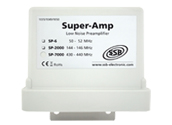
\includegraphics[width=\halftextwidth]{LNA}
\caption{\acl{LNA}}
\label{fig:lna}
\end{figure}



\subsection{Radio}

The radio receiver is important for the proper reception of the satellite signals since it contains a number of filters that eliminate strong terrestrial signals (and their harmonics) from radio sources located at the vicinity of the \GroundStationName~ antennas. The location of the \ac{EWI} building exposes it to a large number of such signal sources, making this issue a point of concern. It is possible to connect the antennas directly to the \ac{SDR} but the neighbouring terrestrial signals may overload the input of the \ac{SDR}, causing intermodulations and a strongly decreased sensitivity. In that case, the weak signals from satellites may be impossible to receive.

The requirements for the radio receiver are:

\begin{itemize*}
\item Reception of satellite's main telemetry downlink frequency bands (\unit{2}{m}, \unit{70}{cm} and S-band);
\item Analogue \ac{IF} output to connect to the \ac{SDR};
\item external reference frequency input;
\item Remote controllable.
\end{itemize*}

Using the radio receiver as a down-converter also opens the possibility of other listening to other frequency bands of interest. Should that prove to be advantageous in the future, there is only the need to acquire the corresponding antenna and \ac{LNA}.

The radio receiver of the \GroundStationName~ is chosen to be the \details{radio}{model}\footnote{Further details: \details{radio}{url}}, see \ref{fig:radio}, with the following relevant characteristics:

\begin{itemize*}
\item Frequency range: \unit{40}{kHz} to \unit{3.15}{GHz};
\item \unit{10}{MHz} reference input (SMA-J connector) for \unit{0.01}{\acs{ppm}} frequency accuracy for the \unit{10}{MHz} internal master oscillator is obtained when synchronized to a \ac{GPS} signal;
\item \unit{45.05}{MHz} Analogue \ac{IF} output with \unit{15}{MHz} bandwidth (BNC-J connector);
\item \ac{USB} 1.1/2.0 connector for \ac{PC} control;
\item remote antenna switching, requires \details{radioswitch}{model}\footnote{Further details:  \details{radioswitch}{url}}.
\end{itemize*}

\begin{figure}[!ht]
\centering
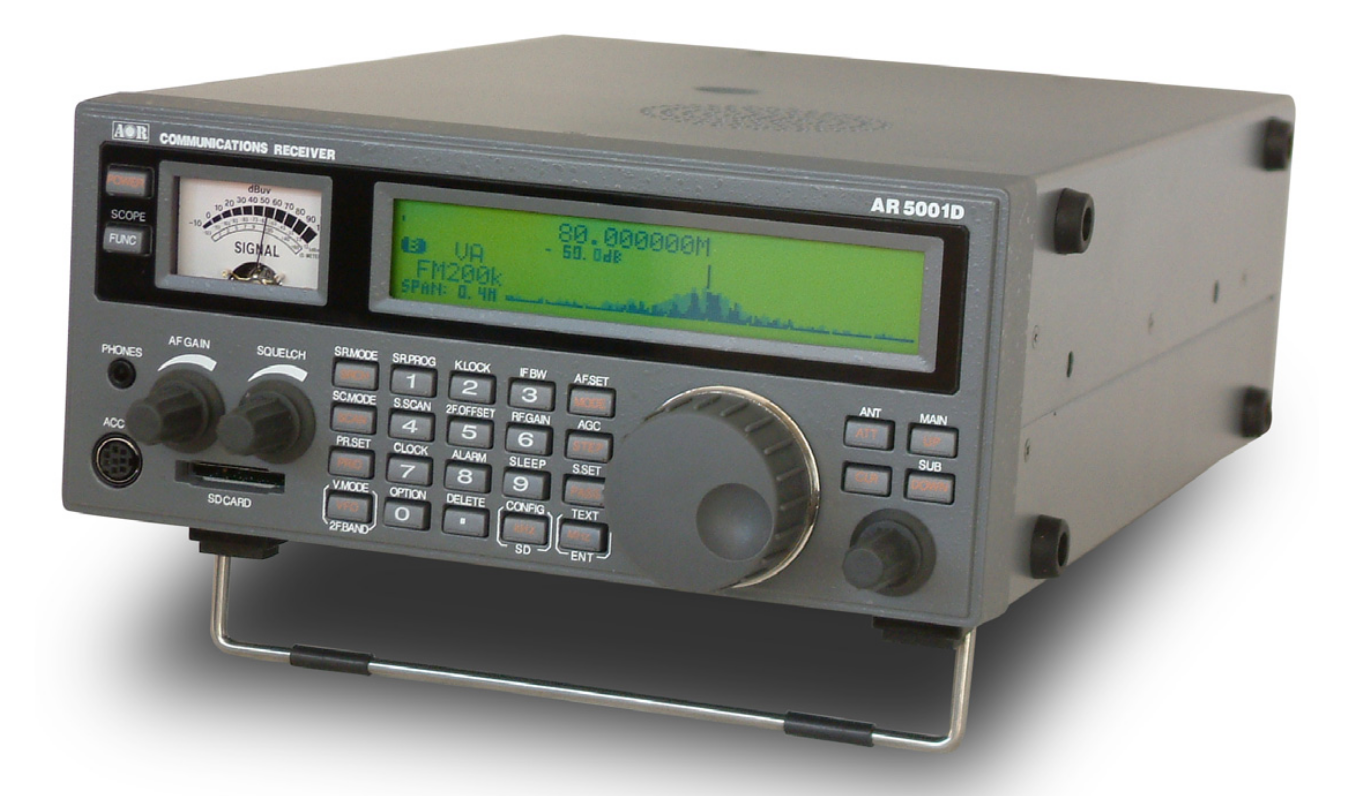
\includegraphics[width=\semitextwidth]{radio}
\caption{Radio receiver}
\label{fig:radio}
\end{figure}



\subsection{\acs{SDR}}

The \ac{SDR} is the key component of the \GroundStationName~ hardware, since it digitalizes the satellite signal to be properly processed. The requirements for the \ac{SDR} are:

\begin{itemize*}
\item High data sampling rate;
\item Open-source Hardware Driver;
\item External reference frequency input;
\item External \ac{pps} input;
\item Remote controllable.
\end{itemize*}

The \ac{SDR} of the \GroundStationName~ is chosen to be the \details{sdr}{model}\footnote{Further details: \details{sdr}{url}}, see \ref{fig:sdr}, with the following relevant characteristics:

\begin{itemize*}
\item \unit{50}{MS/s} streaming rate (upgradable to \unit{100}{MS/s});
\item Gigabit \ac{LAN} Interface to \ac{PC};
\item \unit{10}{MHz} reference frequency input;
\item Dual \unit{100}{MS/s}, \unit{14}{bit} \ac{ADC};
\item based on open-source GNU Radio software;
\item \details{sdrdb}{model} for \unit{1-250}{MHz} reception.
\end{itemize*}

\begin{figure}[!ht]
\centering
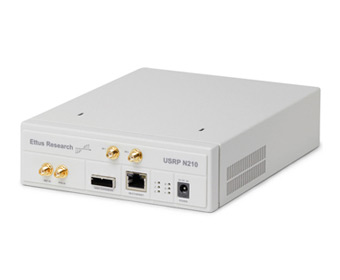
\includegraphics[width=\semitextwidth]{sdr}
\caption{\acl{SDR}}
\label{fig:sdr}
\end{figure}



\subsection{\acs{GPS} disciplined clock}

The clock is responsible for feeding the radio receiver and \ac{SDR} with a \unit{10}{MHz} reference frequency, so that the incoming signal's frequency can be measured accurately. Failing to do so means that the radio and \ac{SDR} will have to resort to the internal (usually Quartz) oscillator to determine the incoming signal's frequency. It is expected at least two orders of magnitude decrease in the frequency stability if the oscillators of the \ac{SDR} and radio receiver are not externally stabilized.

Additionally, double-frequency tropospheric and ionospheric delay correction can only be accomplished if the two hardware streams are synchronized. The clock provides \unit{1}{\acs{pps}} signals that allow for the synchronization of all relevant hardware components, namely the two computers. Additionally, the \ac{pps} signals provides a timing reference to the \ac{SDR} for accurate triggering of the recording session and time-tagging of the measurements.

The requirements for the \acs{GPS} disciplined clock are:

\begin{itemize*}
\item High frequency stability, better than \unit{0.01}{\acs{ppm}}
\item Multiple reference frequency outputs;
\item Multiple \ac{pps} outputs;
\item Remote controllable.
\end{itemize*}

The \acs{GPS} disciplined clock of the \GroundStationName~ is chosen to be the \details{clock}{model}\footnote{Further details: \details{clock}{url}}, see \ref{fig:clock}, with the following relevant characteristics:

\begin{itemize*}
\item \ac{GPS} 12 channel reception on \ac{L1} \ac{C/A-code};
\item \ac{pps} accuracy to \ac{UTC}: \unit{25}{ns} ($1\sigma$);
\item \unit{10}{MHz} accuracy $<$ 2e-12 (one day average);
\item Temperature Stability (peak to peak): 1e-9 (from \unit{0 - 60}{^\circ C});
\item 7 $\times$ \unit{10}{MHz} sine wave outputs;
\item 7 $\times$ \unit{1}{\acs{pps}} outputs;
\item Remote management through Ethernet port;
\item \ac{NTP} server;
\item Full remote control by serial port RS-232C.
\end{itemize*}

\begin{figure}[!ht]
\centering
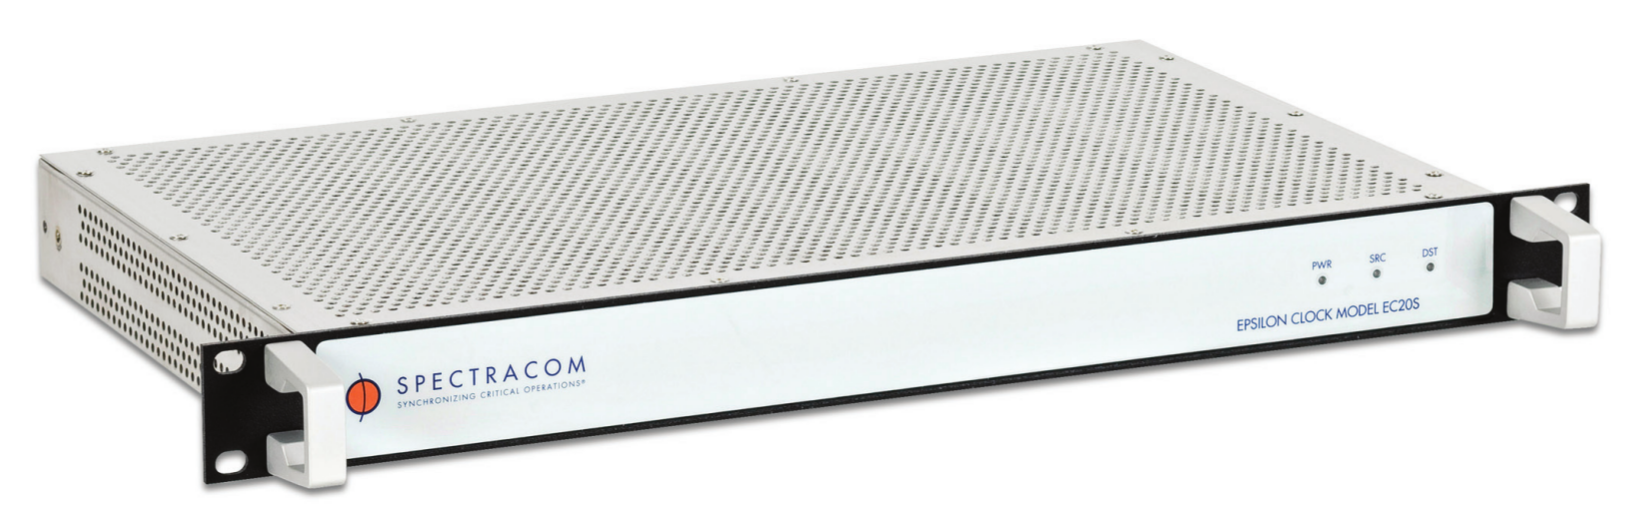
\includegraphics[width=\fulltextwidth]{clock}
\caption{\acs{GPS} disciplined clock}
\label{fig:clock}
\end{figure}



\subsection{Computer}

The \ac{PC} for the \GroundStationName~ does not have particularly strong requirements, since the heavy processing is done in the \ac{SDR}:

\begin{itemize*}
\item Gigabit \ac{LAN} Interface;
\item Able to run Ubuntu \ac{OS};
\item \unit{200-500}{Gb} hard disk.
\end{itemize*}

All these requirements are easily met with an old computer that is not longer in use, which is advantageous to reduce costs.



\subsection{Budget}

The budget of the \GroundStationName~ hardware is summarized in \ref{tab:budget}

\newcommand{\tablerow}[1]{\details{#1}{name} & \details{#1}{model} & \details{#1}{quant} & \details{#1}{price} \\}

\begin{table}[!ht]
\centering
\begin{tabular}{m{4cm}>{\raggedright\arraybackslash}m{4cm}>{\centering\arraybackslash}m{1.50cm}>{\raggedleft\arraybackslash}m{1.5cm}}
% \begin{tabular}{llrc}
\hline
Component & Model & Quantity & Cost (\euro) \\
\hline
% \foreach \item in {lna,radio,radioswitch,sdr,sdrdb,sdrrack,clock,antennaUHF,biasT,lightprot,splitVUHF,splitSband,computer,misc}{
\tablerow{antennaUHF}
\tablerow{lna}
\tablerow{radio}
\tablerow{radioswitch}
\tablerow{sdr}
\tablerow{sdrdb}
\tablerow{computer}
\tablerow{clock}
\tablerow{sdrrack}
\tablerow{misc}
\tablerow{biasT}
\tablerow{lightprot}
\tablerow{splitSband}
\tablerow{splitVUHF}
\tablerow{adapters}
\tablerow{radiorack}
\tablerow{gpsantenna}
% \tablerow{tax}
% \tablerow{deliv}
\hline
\tablerow{hardcost}
\hline
\tablerow{assembly}
\tablerow{maintenance}
\tablerow{TA}
\tablerow{CourseMat}
\hline
\tablerow{total}
\hline
\end{tabular}
\caption{Budget for the \GroundStationName hardware.}
\label{tab:budget}
\end{table}

\clearpage
\section{Software}


The following software is going to be used in order to accomplish the objectives.

\begin{itemize*}
\item Ubuntu\footnote{\url{www.ubuntu.com}} \ac{OS};
\item \ac{BASH} shell and Ruby\footnote{\url{www.ruby-lang.org}} for automation;
\item \ac{MATLAB} or Python\footnote{\url{www.python.org}} for the extraction of the Doppler-shift profiles from the \ac{I/Q} data;
\item \ac{TUDAT} and C++ for the orbit estimation.
\end{itemize*}


\section{Planning}

The following schedule is currently agreed between all intervening \GroundStationName staff.

\begin{description*}
\item[Building station:] September - October 2014;
\item[Testing setup:] November - December 2014;
\item[Course development:] January - March 2015;
\item[Combination with Minor:] May - September 2015.
\end{description*}

\pagebreak
\section{Technical specifications}


The technical specifications of the hardware can be found in the (click-able) web pages listed in \ref{tab:techspecs}.

\renewcommand{\tablerow}[1]{\details{#1}{name} & \details{#1}{url} \\ \hline}

\begin{table}[!ht]
\centering
\begin{tabular}{m{3cm}>{\footnotesize\arraybackslash}m{9cm}}
\hline
Component & Brochure/Technical Specifications \\
\hline
\tablerow{lna}
\tablerow{radio}
\tablerow{radioswitch}
\tablerow{sdr}
\tablerow{sdrdb}
\tablerow{sdrrack}
\tablerow{clock}
\tablerow{antennaUHF}
\tablerow{biasT}
\tablerow{lightprot}
\tablerow{splitVUHF}
\tablerow{splitSband}
\tablerow{computer}
\end{tabular}
\caption{Technical specifications of the \GroundStationName hardware.}
\label{tab:techspecs}
\end{table}



%% ==========================  acronyms =========================== %%

\ifdefined\UseAcronyms
  \ifdefined\IncludeAcronymList
    \newpage
    \section*{Acronyms}
  \fi
  % !TEX root = ./doptrack.budget.tex

%Helper for the definition of acronyms with citations:
%\acrocite{acronym}{long version}{citation key}
%The acronyms defines a citation in the list of acronyms.
%A second acronym called acronym.cite includes the citation in the text.
%example:
%\acrocite{FES2004}{Finite Element Solution model release 2004}{Lyard2006}
%produces:
%\acro{FES2004}{Finite Element Solution model release 2004\acroextra{, \citep{Lyard2006}}}
%\acrodef{FES2004.cite}[!use acl with .cite acronyms!]{Finite Element Solution model release 2004 (FES2004, \citealt{Lyard2006})}
%WARNING: always use \acl with the .cite acronyms!
\ifdefined\UseCitationsInAcronyms
  \ifdefined\UseNatBib
    \newcommand{\acrodefcite}[4][ ]{
      \acrodef{#2.cite}[!use acl with .cite acronyms!]{#3 (#2)#1\protecting{(\citealt{#4})\acused{#2}}}
    }
    \newcommand{\acrocite}[4][ ]{
      \acro{#2}{#3#1\acroextra{, \protecting{\citet{#4}}}}
      \acrodefcite[#1]{#2}{#3}{#4}
    }
  \else
    \newcommand{\acrodefcite}[4][ ]{
      \acrodef{#2.cite}[!use acl with .cite acronyms!]{#3 (#2)#1\protecting{(\citealt{#4})\acused{#2}}
    }
    \newcommand{\acrocite}[4][ ]{
      \acro{#2}{#3#1\acroextra{, \protecting{\citet{#4}}}}
      \acrodefcite[#1]{#2}{#3}{#4}
    }
  \fi
\else
  \newcommand{\acrodefcite}[4][ ]{
    \acrodef{#2.cite}[!use acl with .cite acronyms!]{#3 (#2)#1\protecting{\acused{#2}}}
  }
  \newcommand{\acrocite}[4][ ]{
    \acro{#2}{#3}
    \acrodefcite[#1]{#2}{#3}{#4}
  }
\fi

%Helper for the definition of acronyms with references:
%\acrocite{acronym}{long version}{reference key}
%The acronyms defines a reference in the list of acronyms.
%A second acronym called acronym.ref includes the reference in the text.
%example:
%\acrocite{HRF}{Hill Reference Frame}{sec:hrf}
%produces:
%\acro{HRF}{Hill Reference Frame\acroextra{, \citep{sec:hrf}}}
%\acrodef{HRF.ref}[]{Hill Reference Frame (HRF, \citealt{sec:hrf})}
%WARNING: always use \acl with the .ref acronyms!
\ifdefined\UseReferencesInAcronyms
  \newcommand{\acroref}[3]{
    \acro{#1}{#2\acroextra{, \protecting{\ref{#3}}}}
    \acrodef{#1.ref}[!use acl with .ref acronyms!]{#2 \protecting{(#1, \ref{#3})\acused{#1}}}
  }
\else
  \newcommand{\acroref}[3]{
    \acro{#1}{#2}
    \acrodef{#1.ref}[!use acl with .ref acronyms!]{#2 (#1)\protecting{\acused{#1}}}
  }
\fi
\newcommand{\acrourl}[3]{
  \acro{#1}{#2\acroextra{, \protecting{\url{#3}}}}
  \acrodef{#1.url}[!use acl with .url acronyms!]{#2 \protecting{(#1, \url{#3})\acused{#1}}}
  \acrodef{#1.urlonly}[!use acl with .urlonly acronyms!]{\protecting{\url{#3}}}
}
\newcommand{\acrourlc}[4]{
  \acro{#2}[#1]{#3\acroextra{, \protecting{\url{#4}}}}
  \acrodef{#2.url}[!use acl with .url acronyms!]{#3 \protecting{(#2, \url{#4})\acused{#2}}}
  \acrodef{#2.urlonly}[!use acl with .urlonly acronyms!]{\protecting{\url{#4}}}
}

\acresetall
\begin{acronym}[-------------------]
%don't use \ace, \act or \acf with acronyms that include a \citep command
%#
\acro{1D}{uni-dimensional}
\acro{2D}{bi-dimensional}
\acro{3D}{three-dimensional}
%A
\acro{AA}{Acceleration Approach}
\acro{ACC}{Accelerometer}
\acro{ASCR}{Academy of Sciences of the Czech Republic}
\acro{ACS}{Attitude Control System}
\acro{ADC}{Analogue-to-Digital Converter}
\acro{AGU}{American Geophysical Union}
\acro{AIL}{Action Item List}
\acrourl{AIUB}{Astronomical Institute of the University of Bern}{http://www.aiub.unibe.ch/}
\acrocite{AIUB-GRACE02S}{\acl{AIUB} \acs{GRACE}-only model, version 2}{Jaggi2012}
\acro{AOCS}{Attitude and Orbital Control System}
%TODO : go throught the text and make sure any \ac{AOD1B} instances is followed by 'product'.
\acrocite[ product ]{AOD1B}{Atmosphere and Ocean De-aliasing \acl{L1B}}{Flechtner2006,Flechtner2007,Flechtner2011}
\acrocite{AOTIM-5}{Arctic Ocean Tidal Inverse Model}{Padman2010}
\acro{ANGARA}{Analysis of Non-Gravitational Accelerations due to Radiation pressure and Aerodynamics}
\acro{AO}{Annoucement of Opportunity}
\acro{ARMA}{Auto-Recursive Moving Average}
\acro{AS}{Anti-Spoofing}
\acro{ASCII}{American Standard Code for Information Interchange}
\acro{ASM}{Astrodynamics and Space Missions\acroextra{, Faculty of Aerospace Engineering, T.U. Delft}}
\acrourl{ASU}{Astronomical Institute\acroextra{ (Astronomick\'y \'ustav), \acs{ASCR}}}{www.asu.cas.cz/en}
%B
\acrourl{BASH}{Bourne-again shell}{www.gnu.org/software/bash}
\acrocite{BDNSS}{BeiDou\slash Compass Navigation Satellite System}{Chengzhi2013}
\acrourl{BIT}{Beijing Institute of Technology}{english.bit.edu.cn}
%C
\acro{C/A-code}{Coarse\slash Acquisition code}
\acro{CAD}{Computer-Aided Design}
\acrocite{CADA00.10}{Circum-Antarctic Tidal Simulation Inverse Model}{Padman2010a}
\acro{Cal/Val}{Calibration and Validation}
\acro{COAS}{College of Oceanic and Atmospheric Sciences\acroextra{, Oregon State University}}
\acro{CCDB}{Characterisation and Calibration Database}
\acrourl{CDF}{Common Data Format}{cdf.gsfc.nasa.gov}
\acrourl{CERGA}{Centre d'\'{e}tudes et de Recherches en G\'{e}odynamique et Astrom\'{e}trie}{wwwrc.obs-azur.fr/cerga/CERGA_anglais.html}
\acro{CLS}{Collecte Localisation Satellites}
\acrocite{CHAMP}{CHallenging Mini-Satellite Payload}{Reigber1996,Reigber2002}
\acrocite{CMA}{Celestial Mechanics Approach}{Beutler2010a}
\acro{CNES}{Centre National d'\'{E}tudes Spatiales}
\acro{COM}{Centre of Mass}
\acrocite{CICERO}{Community Initiative for Continuing Earth Radio Occultation}{GeoOptics2013}
\acrocite{CNES/GRGS-10d}{\acl{CNES}\slash\acl{GRGS} 10-days gravity field models}{Bruinsma2010}
\acro{COSMIC}{Constellation Observing System for Meteorology, Ionosphere and Climate\acroextra{ (see  also \acs{F3C})}} %reference added to F3C.cite
\acro{COSMIC-2}{2nd Constellation Observing System for Meteorology, Ionosphere and Climate\acroextra{ (see also \acs{F7C2})}} %reference added to F3C.cite
\acro{COTS}{Commercial Off-The-Shelf}
\acro{CPR}{Cycle Per Revolution}
\acrodefplural{CPR}{Cycles Per Revolution}
\acrourl{CSR}{Center for Space Research\acroextra{, The University of Texas at Austin, \acs{USA}}}{www.csr.utexas.edu}
\acrocite{CSR3.0}{version 3 of the \acs{CSR}'s global ocean model}{Eanes1996}
\acrocite{CSR4.0}{version 4 of the \acs{CSR}'s global ocean model}{Eanes1999}
\acroref{CRF}{Celestial Reference Frame}{sec:crf} %if you change this, also change the superscript
\acrodef{CV}{Curriculum Vit\ae}
\acrodefplural{CV}{Curricula Vit\ae}
%D
\acro{DAS}{degree amplitude spectrum}
\acrodefplural{DAS}{degree amplitude spectra}
\acro{DD}{Double-differenced}
\acrocite{DEMETER}{Development of a European Multimodel Ensemble system for seasonal to inTERannual prediction}{Palmer2004}
\acro{DEOS}{Delft Institute for Earth-Oriented Space research}
\acro{DFACS}{Drag-Free Attitude Control Systems}
\acro{DLR}{Deutsches Zentrum f\"ur Luft- und Raumfahrt}
\acro{DGFI}{Deutsches Geod\"atisches Forschungsinstitut}
%TODO : go throught the text and make sure any \ac{DMT-1} instances is followed by 'product'.
\acrocite{DMT-1}{Delft Mass Transport}{Liu2010}
\acro{DOF}{Direction Of Flight}
\acrocite{DORIS}{Doppler Orbit Determination and Radio-positioning Integrated on Satellite}{Dorrer1991,Barlier2005,Willis2006}
\acro{DOWR}{Dual One-Way Ranging}
\acro{DOY}{Day Of Year}
\acrocite{DTM}{Drag Temperature Model}{Bruinsma2003}
\acrocite{DW95.1}{Desai-Wahr global ocean model}{Desai1995,Desai1997}
%E
\acro{E2E}{End-to-End}
\acro{ECEF}{Earth-Centred, Earth-Fixed}
\acro{ECI}{Earth-Centred Inertial}
\acro{EFRF}{Earth-Fixed Reference Frame}
\acrocite{ECMWF}{European Centre for Medium-Range Weather Forecasts}{ECMWF2011}
\acrocite{EGM2008}{U.S. National Geospatial-Intelligence Agency's Earth Gravitational Model 2008}{Pavlis2008}
\acrocite{EIGEN-CG03C}{GeoForschungsZentrum Potsdam\slash Groupe de Recherche de G\`eod\'esie Spatiale combined gravity field model, version 3}{Forste2005}
\acrocite{EIGEN-GL04C}{GeoForschungsZentrum Potsdam\slash Groupe de Recherche de G\`eod\'esie Spatiale combined gravity field model, version 4}{Forste2008}
\acrocite{EIGEN-GRACE02S}{GeoForschungsZentrum Potsdam\slash Groupe de Recherche de G\`eod\'esie Spatiale \acs{GRACE}-only gravity field model, version 2}{Reigber2005}
\acrocite{EIGEN-5C}{GeoForschungsZentrum Potsdam\slash Groupe de Recherche de G\`eod\'esie Spatiale combined gravity field model, version 5}{Forste2008a}
\acro{EGG}{Electrostatic Gravity Gradiometer}
\acro{EGU}{European Geophysical Union}
\acro{EKF}{Extended Kalman Filter}
\acro{ENSS}{European Navigation Satellites Services}
\acro{ENVISAT}{ENVIronmental SATellite} %need reference
\acrocite{EOT08a}{2008 Empirical Ocean Tide model derived from Altimeter data}{Savcenko2008,Savcenko2008a}
\acro{EWH}{equivalent water height}
\acro{EWI}{Elektrotechniek, Wiskunde en Informatica\acroextra{ faculteit (Faculty of Electrical Engineering, Mathematics and Computer Science), TU Delft}}
\acro{EO}{Earth Observation}
\acrocite{ERS-1}{First European Remote Sensing satellite}{Duchossois1991}
\acrocite{ERS-2}{Second European Remote Sensing satellite}{Francis1995}
\acrocite{ERA-40}{40-years ECMWF Re-Analysis}{Uppala2005}
\acrocite{ERA-Interim}{\quotes{Interim} ECMWF Re-Analysis}{Dee2011,Berrisford2011}
\acro{ESRL}{Earth System Research Laboratory\acroextra{ part of \acs{NOOA}}}
\acrourl{ESA}{European Space Agency}{www.esa.int}
\acrourl{ESOC}{European Space Agency}{www.esa.int/About\_Us/ESOC}
\acrourl{ESTEC}{European Space Research and Technology Centre}{www.esa.int/About\_Us/ESTEC}
\acro{EU}{European Union}
%F
\acrocite{F3C}{\acs{FORMOSAT-3}\slash \acs{COSMIC}}{Kuo1999,Kuo2005}
\acrocite{F7C2}{\acs{FORMOSAT-7}\slash \acs{COSMIC-2}}{Ector2010,Cook2013}

\acro{FDDW}{Frequency-Dependent Data Weighting}
\acro{FES}{Finite Element Solution\acroextra{ global tide model}}
\acrocite[ global tide model ]{FES94.1}{release 1994 of the \acl{FES}}{LeProvost1994}
\acrocite[ global tide model ]{FES95.2}{release 1995 of the \acl{FES}}{LeProvost1998}
\acrocite[ global tide model ]{FES99}  {release 1999 of the \acl{FES}}{Lefevre2002}
\acrocite[ global tide model ]{FES2004}{release 2004 of the \acl{FES}}{Lyard2006}
\acro{FRT}{Final Report}
\acro{FORMOSAT-3}{Taiwan's Formosa Satellite Mission-3\acroextra{ (see also \acs{F3C})}} %reference added to F3C.cite
\acro{FORMOSAT-7}{Taiwan's Formosa Satellite Mission-7\acroextra{ (see also \acs{F7C2})}} %reference added to F7C2.cite
\acro{FORTRAN}{FORmular TRANslator\acroextra{ programing languange}}
%G
\acro{GB}{Giga Bytes\acroextra{, i.e. $1024\times1024\times1024$ bytes}}
\acro{GEOSAT}{GEOdetic SATellite} %need reference
\acro{GEOSAT-FO}{\acs{GEOSAT} Follow-On} %need reference
\acrocite{GFO}{\acs{GRACE} Follow On}{Larkin2012,Zaragoza2013}
\acrourl{GFZ}{Helmholtz-Zentrum Potsdam Deutsches GeoForschungsZentrum}{www.gfz-potsdam.de}
\acro{GHOST}{GPS High precision Orbit determination Software Tool}
\acrocite{GGM02}{GRACE Gravity Model 02}{Tapley2005}
\acrocite{GGM03}{GRACE Gravity Model 03}{Tapley2007a}
\acro{GIA}{Glacial Isostatic Adjustment}
\acrocite{GLDAS}{Global Land Data Assimilation System}{Rodell2004}
\acrocite{GLONASS}{Globalnaya Navigatsionnaya Sputnikovaya Sistema}{Polischuk2004} %need reference
\acro{GNSS}{Global Navigation Satellite System}
\acrocite{GOCE}{Gravity field and steady-state Ocean Circulation Explorer}{Balmino1999,Floberghagen2011} %need reference
\acrocite{GOCO01S}{Gravity Observation COmbination release 01 satellite-only gravity field model}{Pail2010}
\acrocite{GOCO02S}{Gravity Observation COmbination release 02 satellite-only gravity field model}{Goiginger2011}
\acrocite{GOCO03S}{Gravity Observation COmbination release 03 satellite-only gravity field model}{Mayer-Gurr2012}
\acrocite{GOT}{Goddard Ocean Tide\acroextra{ model}}{Ray1999}
\acro{GPS}{Global Positioning System}
\acrocite{GRACE}{Gravity Recovery And Climate Experiment}{Tapley1996,Tapley2004}
\acrocite{GRAIL}{Gravity Recovery and Interior Laboratory\acroextra{ mission}}{Lehman2013}
\acrocite{GRAPHIC}{Group and Phase Ionospheric Calibration}{Montenbruck2003a}
\acro{GRAS}{Global navigation Receiver for Atmospheric Sounding} %need reference
\acroref{GRF}{Gradiometer Reference Frame}{sec:grf} %if you change this, also change the superscript
\acrourl{GRS}{Geoscience and Remote Sensing}{www.citg.tudelft.nl/over-faculteit/afdelingen/geoscience-and-remote-sensing}
\acrocite{GRIB}{GRIdded Binary}{NWS2010}
\acro{GRGS}{Groupe de Recherche de G\'{e}od\'{e}sie Spatiale}
\acro{GSFC}{Goddard Space Flight Center}
%H
\acrocite{HASDM}{High Accuracy Satellite Drag Model}{Storz2005}
\acroref{HRF}{Hill Reference Frame}{sec:hrf}
\acro{hlsst}[hl-SST]{High-low Satellite-to-Satellite tracking}
\acro{HPF}{High-Level Processing Facility}
\acro{HTG}{Hypersonic Technology Goettingen\acroextra{ (Hyperschall Technologie G\"ottinge GmbH)}}
\acro{HTTP}{Hypertext Transfer Protocol}
\acro{HWM07}{Horizontal Wind Model 07}
%I
\acro{IAG}{International Association of Geodesy}
\acro{IAU}{International Astronomical Union}
\acro{ICET}{International Center for Earth Tides}
\acro{ICESat}{Ice, Cloud and land Elevation Satellite} %need reference
\acrourl{ICGEM}{International Centre for Global Earth Models}{icgem.gfz-potsdam.de}
\acro{IERS}{International Earth Rotation Service}
\acro{IF}{Intermediate Frequency}
\acrocite{IGS}{International \acs{GNSS} Service}{Dow2005}
\acro{InSAR}{Interferometric Synthetic Aperture Radar}
%Iridium NEXT \citep{Gupta2008} %there is no acronym for this, so cannot use \acrocite
\acro{I/Q}{In-phase\slash Quadrature}
\acro{IRF}{Inertial Reference Frame}
\acro{ISA}{In-situ Accelerations}
\acro{ISR}{Inter-Satellite Range}
\acrourl{IST}{Instituto Superior T\'ecnico}{tecnico.ulisboa.pt}
\acro{ITAM}{Institute of Theoretical and Applied Mechanics, \acs{ASCR}}
\acrourl{ITG}{Institut f\"ur Geod\"asie und Geoinformation}{www.igg.uni-bonn.de}
\acrocite{ITG-CHAMP01}{\acl{ITG} \acs{CHAMP}-only model, version 1}{Mayer-Gurr2005}
\acrocite{ITG-GRACE2010}{\acl{ITG} \acs{GRACE}-only model, 2010}{Mayer-Gurr2010}
\acrourl{ITRF}{International Terrestrial Reference Frame}{itrf.ensg.ign.fr}
\acro{ITT}{Invitation To Tenders}
%J
\acrocite{Jason-1}{First Jason altimetry mission}{Menard2003}
\acrourl{JPL}{Jet Propulsion Laboratory}{www.jpl.nasa.gov}
%K
\acrocite{KANTHA2}{Khanta global ocean model}{Kantha1995,Kantha1995a}
\acro{KBR}{K-Band Ranging}
\acro{KO}{Kinematic Orbit}
\acro{K/O}{Kick Off}
%L
\acro{L0}{Level 0\acroextra{ data}}
\acro{L1}{\unit{1575.42}{mHz} \acs{GPS} carrier\acroextra{ frequency}}
\acro{L1data}[L1]{Level 1\acroextra{ data}}
\acro{L1A}{Level 1A\acroextra{ data}}
\acro{L1B}{Level 1B\acroextra{ data}}
\acro{L2}{\unit{1227.60}{mHz} \acs{GPS} carrier\acroextra{ frequency}}
\acro{L2data}[L2]{Level 2\acroextra{ data}}
\acro{L2PS}{Level 2 Processing System}
\acro{L5}{\unit{1176.45}{mHz} \acs{GPS} carrier\acroextra{ frequency}}
\acro{LAN}{Local Area Network}
\acro{LAGEOS}{LAser GEOdynamics Satellite} %need reference
\acro{LASER}{Light Amplification by the Stimulated Emission of Radiation}
\acrourl{latex}{\LaTeX}{www.latex-project.org}
\acro{LEGOS}{Laboratoire d'Etudes en Geophysique et Oceanographie Spatiale}
\acro{LEO}{Low-Earth Orbit}
\acroref{LHRF}{Local Horizontal Reference Frame}{sec:lhrf} %if you change this, also change the superscript
\acrourlc{Lic. Eng.}{LicEng}{Licenciatura em Engenharia\acroextra{ (Licenciate in Engineering, pre-Bologna Accords)}}{en.wikipedia.org/wiki/Licentiate\#Portugal}
\acrocite{LISA}{Laser Interferometer Space Antenna}{Merkowitz2003}
\acro{llsst}[ll-SST]{Low-low Satellite-to-Satellite tracking}
\acro{LNA}{Low-Noise Amplifier}
\acro{LNOF}{Local North-Oriented Frame}
\acroref{LORF}{Local Orbital Reference Frame}{sec:lorf} %if you change this, also change the superscript
\acro{LOS}{Line-of-Sight} %if you change this, also change uv.los
\acroref{LOSRF}{Line-of-sight Reference Frame}{sec:losrf} %if you change this, also change the superscript
\acro{LNA}{Low-Noise Amplifier}
%M
\acrourl{MATLAB}{MATrix LABoratory}{www.mathworks.com}
\acro{MB}{Mega Bytes\acroextra{, i.e. $1024\times1024$ bytes}}
\acrocite{MetOp}{Meteorological Operational satellite programme}{Edwards2000}
\acro{MetOp-A}{first satellite of the \acl{MetOp}} %need reference
\acro{MPP}{Milestone Payment Plan}
\acro{MTR}{Mid-Term Review}
\acro{FR}{Final Review}
%N
\acro{N/A}{Not Applicable}
\acro{NASA}{National Aeronautics and Space Administration}
\acro{NAO}{National Astronomical Observatory\acroextra{, Japan}}
\acrocite{NAO.99b}{1999 release of the \acs{NAO}'s global ocean model}{Matsumoto2000}
\acro{NAVSTAR}{NAVigation System with Time And Ranging} %need reference
\acro{NCAR}{National Center for Atmospheric Research}
\acrocite{NCEP/NCAR RP}{\acs{NCEP}/\acs{NCAR} Reanalysis Project}{Kalnay1996}
\acro{NCEP}{National Centers for Environmental Prediction}
\acrocite{NetCDF}{Network Common Data Form}{Unidata2010}
\acro{NLDAS}{North American Land Data Assimilation System}
\acro{NOOA}{National Oceanic and Atmospheric Administration}
\acro{NRTDM}{Near Real-Time Density Model}
\acrourl{NTP}{Network Time Protocol}{www.ntp.org}
%O
\acrourl{OCA}{Observatoire de la C\^{o}te d'Azur}{www.oca.eu}
\acrocite{OMCT}{Ocean Model for Circulation and Tides}{Thomas2001}
\acro{ORI}{Ocean Research Institute\acroextra{, University of Tokyo}}
\acrocite{ORI-NAO96}{1996 release of the \acs{ORI}-\acs{NAO}'s global ocean model}{Matsumoto1995}
\acro{OS}{Operating System}
%P
\acro{P-code}{Precision code}
\acrocite{PANDA}{Position And Navigation Data Analyst\acroextra{ software}}{Zhao2004}
\acro{PC}{Personal Computer}
\acro{PCCG}{Pre-Conditioned Conjugate Gradient}
\acrourl{PDF}{Portable Data Format}{en.wikipedia.org/wiki/Portable_Document_Format}
\acro{PDGS}{Payload Data Ground Segment}
\acro{PDO}{Purely Dynamic Orbit}
\acrourl{PECS}{Programme for European Cooperating States}{www.esa.int/About_Us/Plan_for_European_Cooperating_States}
\acro{PM}{Progress Meeting}
\acro{POD}{Precise Orbit Determination}
\acrocite{PO.DAAC}{Physical Oceanography Distributed Active Archive Center}{PODAAC2011}
\acro{ppm}{parts per million}
\acro{PPS}{Precise Positioning Service}
\acro{pps}{pulse per second}
\acro{PRN}{Pseudo-Random Noise}
\acro{PSD}{Power Spectral Density}
\acro{PSK}{Phase-Shift Keying}
\acro{PSO}{Precise or Post-processed Science Orbit}
\acro{PSS}{Procedures Specifications and Standards}
%Q
\acro{QWG}{Quality Working Group}
%R
\acrourl{RADS}{Radar Altimeter Database System}{rads.tudelft.nl}
\acro{RDO}{Reduced Dynamic Orbit}
\acro{RF}{Radio Frequency}
\acro{RINEX}{Receiver Independent Exchange\acroextra{ Format}}
\acrocite{RossInv2002}{Ross Sea Height-Based Tidal Inverse Model}{Padman2010b}
\acro{RMS}{Root Mean Squared}
\acro{RRC}{Residual Range Combinations}
\acrocite{RSC94}{\acs{GSFC} Ray-Sanchez-Cartwright global ocean model}{Cartwright1991}
%S
\acro{SA}{Selective Availability}
\acro{S/C}{spacefract}
\acrocite{SCARF}{Swarm Satellite Constellation Application and Research Facility}{Olsen2013a}
\acro{SCP}{Secure Copy}
\acro{SD}{Single-Differenced}
\acro{SD-E}{\acl{SD} phase measurements between Epochs}
\acro{SD-S}{\acl{SD} phase measurements between \acs{GPS} Satellites}
\acro{SDR}{Software Defined Radio}
\acro{SFTP}{Secure File Transfer Protocol}
\acro{SGG}{Satellite Gravity Gradient}
\acro{SG}{Satellite Gradiometry}
\acrocite{SLR}{Satellite Laser Ranging}{Smith1993,Combrinck2010}
\acro{SOW}{Statement of Work}
\acrourl{SP3c}{Extended Standard Product 3 Orbit Format}{igscb.jpl.nasa.gov/igscb/data/format/sp3c.txt}
\acro{SPOT}{Satellite Pour l’Observation de la Terre}
\acro{SPS}{Standard Positioning Service}
\acro{SNR}{Signal-to-Noise Ratio}
\acrocite{SR95.1}{T.U. Delft/\acs{GSFC} Schrama-Ray global ocean models}{Schrama1994}
\acroref{SRF}{Satellite Reference Frame}{sec:srf} %if you change this, also change the superscript
\acro{SRTM}{Shuttle Radar Topographic Mission} %need reference
\acrourl{SSAU}{Samara State Aerospace University}{www.ssau.ru/english}
\acro{SSE}{Space Systems Engineering\acroextra{ group of the Faculty of Aerospace Engineering, TU Delft}}
\acro{SSO}{Sun-Synchronous Orbit}
\acro{SST}{Satellite-to-Satellite tracking}
\acro{STD}{standard deviation}
\acrocite{Swarm}{The Earth's Magnetic Field and Environment Explorers}{Friis-Christensen2006}
\acro{STSE}{Support to Science Element}
\acro{STR}{star tracker}
\acrourl{SVN}{Subversion}{subversion.apache.org}
\acrocite{SCW80}{Schwiderski global tide model}{Schwiderski1980,Schwiderski1980a}
%T
%\acro{TA}{True Anomaly}
\acro{TA}{Teaching Assistant}
\acro{TBA}{To Be Announced}
\acro{TBD}{To Be Determined}
\acro{TC}{Trailing\slash Cartwheel}
\acro{TD}{Triple-differenced}
\acro{TDP}{Technical Data Package}
\acrourl{TDRSS}{Tracking and Data Relay Satellite System}{tdrs.gsfc.nasa.gov}
\acro{TDW}{Thermospheric Density and Wind}
\acrourl{TLE}{Two-Line Elements}{www.space-track.org}
\acro{TOPEX}{TOPography EXperiment}
\acrocite{TOPEX/Poseidon}{\acs{TOPEX}\slash Poseidon}{Stewart1981}
\acrocite{TPXO}{ToPeX Ocean tidal model}{Egbert1994,Egbert2002}
\acroref{TRF}{Terrestrial Reference Frame}{sec:trf} %if you change this, also change the superscript
\acro{TS}{Trailing\slash Screw}
\acro{TT}{Terrestrial Time}
\acrourl{TUDAT}{TU Delft Astrodynamics Toolbox}{tudat.tudelft.nl}
\acrourlc{TU Delft}{TUD}{Delft University of Technology}{www.tudelft.nl}
\acrocite{TUM-2Sp}{Technische Universit\"at M\"unchen 2Sp\acroextra{ gravity field model}}{Foldvary2004}
%U
\acro{UHF}{Ultra High Frequency\acroextra{ band of the \acs{RF} spectrum}}
\acro{UTC}{Coordinated Universal Time}
\acro{USA}{United States of America}
\acro{USB}{Universal Serial Bus}
%V
\acro{V2}{Version 2\acroextra{ of the \acs{L2PS}}}
\acro{VHF}{Very High Frequency\acroextra{ band of the \acs{RF} spectrum}}
\acrourl{VZLU}{Aeronautical Research and Test Institute\acroextra{ (V\'yzkumn\'y a zku\u sebn\'i leteck\'y \'ustav)}}{www.vzlu.cz/en}
%X
%W
\acro{WAV}{Windows Wave\acroextra{ file format}}
\acro{WBS}{Work Breakdown Structure}
\acrocite{WGHM}{Watergap Global Hydrological Model}{Doll2003}
\acrocite{WGS84}{World Geodetic System 1984}{Mularie2000}
\acro{WP}{Work Package}
%Y
%Z
\acro{ZD}{Zero-differenced}
\end{acronym}

\acresetall
\fi

%% ==========================  symbols =========================== %%

\ifdefined\UseSymbols
  \ifdefined\IncludeAcronymList
    \newpage
    \section*{Symbols}
  \fi
  % !TEX root = ./doptrack.budget.tex

%TODO: try \ensuremath to all of these, instead of $...$

%% ======================== flexible olerloading of plural forms of acronyms ========================== %%

%\acro and \acrodef derivatives that also define a plural form with the same label
\newcommand*{\acrosympluralbase}[5]{
	\acro			{#1}			[#2]{#3}
	\acroplural		{#1}			[#4]{#5}
}
\newcommand*{\acrodefsympluralbase}[5]{
	\acrodef		{#1}	[#2]{#3}
	\acrodefplural	{#1}	[#4]{#5}
}

%% ======================== overloading 'at epoch i' forms of acronyms ========================== %%

%when in IncludeListWithAllSymbolForms, print the list of symbols with all symbols, including plurals and $_i$ forms
\ifdefined\IncludeListWithAllSymbolForms

%\acro and \acrodef derivatives cumulative with \acrosympluralbase that also define the suffixes $_i$ in the short form and "at epoch i" in the long form.
\newcommand*{\acrosymplural}[5]{
	\acrosympluralbase		{#1}	{#2}		{#3}				{#4}		{#5}				(\acsp{#1}   \aclp{#1})   {\sf \bf #1}
	\acrosympluralbase		{#1.i}	{#2$_i$}	{#3 at epoch $i$}	{#4$_i$}	{#5 at epoch $i$}	(\acsp{#1.i} \aclp{#1.i}) {\sf \bf #1.i}
}
\newcommand*{\acrodefsymplural}[5]{
	\acrosympluralbase		{#1}	{#2}		{#3}				{#4}		{#5}				(\acsp{#1}   \aclp{#1})   {\sf \bf #1}
	\acrosympluralbase		{#1.i}	{#2$_i$}	{#3 at epoch $i$}	{#4$_i$}	{#5 at epoch $i$}	(\acsp{#1.i} \aclp{#1.i}) {\sf \bf #1.i}
}
%\acro and \acrodef derivatives cumulative with \acrosympluralbase that also DON'T define the suffixes $_i$ in the short form and "at epoch i" in the long form.
\newcommand*{\acrosympluralni}[5]{
	\acrosympluralbase		{#1}	{#2}		{#3}				{#4}		{#5}				(\acsp{#1}   \aclp{#1})   {\sf \bf #1}
}
\newcommand*{\acrodefsympluralni}[5]{
	\acrosympluralbase		{#1}	{#2}		{#3}				{#4}		{#5}				(\acsp{#1}   \aclp{#1})   {\sf \bf #1}
}

%when not in IncludeListWithAllSymbolForms, print the list of symbols with only the top symbols and no plurals and $_i$ forms
\else

%\acro and \acrodef derivatives cumulative with \acrosympluralbase that also define the suffixes $_i$ in the short form and "at epoch i" in the long form.
\newcommand*{\acrosymplural}[5]{
	\acrosympluralbase		{#1}	{#2}		{#3}				{#4}		{#5}
	\acrodefsympluralbase	{#1.i}	{#2$_i$}	{#3 at epoch $i$}	{#4$_i$}	{#5 at epoch $i$}
}
\newcommand*{\acrodefsymplural}[5]{
	\acrodefsympluralbase	{#1}	{#2}		{#3}				{#4}		{#5}
	\acrodefsympluralbase	{#1.i}	{#2$_i$}	{#3 at epoch $i$}	{#4$_i$}	{#5 at epoch $i$}
}
%\acro and \acrodef derivatives cumulative with \acrosympluralbase that also DON'T define the suffixes $_i$ in the short form and "at epoch i" in the long form.
\newcommand*{\acrosympluralni}[5]{
	\acrosympluralbase		{#1}	{#2}		{#3}				{#4}		{#5}
}
\newcommand*{\acrodefsympluralni}[5]{
	\acrodefsympluralbase	{#1}	{#2}		{#3}				{#4}		{#5}
}

\fi

%% ======================== olerloading 'at epoch i' and plural forms of acronyms ========================== %%

%\acro and \acrodef derivatives cumulative with \acrosymplural that replicate the short and long forms, appending "s" after the long form
\newcommand*{\acrosym}			[3]{\acrosymplural		{#1}{#2}{#3}{#2}{#3s}}
\newcommand*{\acrodefsym}		[3]{\acrodefsymplural	{#1}{#2}{#3}{#2}{#3s}}

%\acro and \acrodef derivatives cumulative with \acrosympluralni that replicate the short and long forms, WITHOUT the "at epoch i" variation
\newcommand*{\acrosymni}		[3]{\acrosympluralni	{#1}{#2}{#3}{#2}{#3s}}
\newcommand*{\acrodefsymni}	[3]{\acrodefsympluralni	{#1}{#2}{#3}{#2}{#3s}}

%\acro and \acrodef derivatives cumulative with \acrosymplural that replicate the short and long forms, WITHOUT appending "s" after the long form
\newcommand*{\acrosymnp}		[3]{\acrosymplural		{#1}{#2}{#3}{#2}{#3}}
\newcommand*{\acrodefsymnp}	[3]{\acrodefsymplural	{#1}{#2}{#3}{#2}{#3}}

%\acro and \acrodef derivatives cumulative with \acrosympluralni that replicate the short and long forms, WITHOUT "at epoch i" variation and "s" after the long form
\newcommand*{\acrosymnip}		[3]{\acrosympluralni	{#1}{#2}{#3}{#2}{#3}}
\newcommand*{\acrodefsymnip}	[3]{\acrodefsympluralni	{#1}{#2}{#3}{#2}{#3}}


%\acro and \acrodef derivatives cumulative with \acrosym that creates a composite symbol and appends "s" after the long form
\newcommand*{\acrocomp}			[2]{\acrosym		{#1.#2}{\acs {#1}\acs{#2}}{\acl{#2} \acl {#1}}}
\newcommand*{\acrodefcomp}		[2]{\acrodefsym		{#1.#2}{\acs {#1}\acs{#2}}{\acl{#2} \acl {#1}}}

%\acro and \acrodef derivatives cumulative with \acrosymni that creates a composite symbol, WITHOUT the "at epoch i" variation
\newcommand*{\acrocompni}		[2]{\acrosymni		{#1.#2}{\acs {#1}\acs{#2}}{\acl{#2} \acl {#1}}}
\newcommand*{\acrodefcompni}	[2]{\acrodefsymni	{#1.#2}{\acs {#1}\acs{#2}}{\acl{#2} \acl {#1}}}

%\acro and \acrodef derivatives cumulative with \acrosymnp that creates a composite symbol and DOESN'T append "s" after the long form
\newcommand*{\acrocompnp}		[2]{\acrosymnp		{#1.#2}{\acs {#1}\acs{#2}}{\acl{#2} \acl {#1}}}
\newcommand*{\acrodefcompnp}	[2]{\acrodefsymnp	{#1.#2}{\acs {#1}\acs{#2}}{\acl{#2} \acl {#1}}}

%\acro and \acrodef derivatives cumulative with \acrosymnip that creates a composite symbol, WITHOUT the "at epoch i" variation and "s" after the long form
\newcommand*{\acrocompnip}		[2]{\acrosymnip		{#1.#2}{\acs {#1}\acs{#2}}{\acl{#2} \acl {#1}}}
\newcommand*{\acrodefcompnip}	[2]{\acrodefsymnip	{#1.#2}{\acs {#1}\acs{#2}}{\acl{#2} \acl {#1}}}

%% ======================== overloading 'xyz-component of the' forms of acronyms ========================== %%

%\acrodef derivatives cumulative with \acrodefsymplural that generate "x,y,z components of the #2 #1", using the long plural forms
\newcommand*{\acrodefcompvec}[2]{
  \acrodefsymplural  {#1.x.#2}  {\acs{#1}\acs{x}\acs{#2}}{\acl{x} of the \acl{#2} \acl {#1}}
                              {\acs{#1}\acs{x}\acs{#2}}{\acl{x} of the \acl{#2} \aclp{#1}}
  \acrodefsymplural  {#1.y.#2}  {\acs{#1}\acs{y}\acs{#2}}{\acl{y} of the \acl{#2} \acl {#1}}
                              {\acs{#1}\acs{y}\acs{#2}}{\acl{y} of the \acl{#2} \aclp{#1}}
  \acrodefsymplural  {#1.z.#2}  {\acs{#1}\acs{z}\acs{#2}}{\acl{z} of the \acl{#2} \acl {#1}}
                              {\acs{#1}\acs{z}\acs{#2}}{\acl{z} of the \acl{#2} \aclp{#1}}
}
%\acrodef derivatives cumulative with \acrodefsymplural that generate "x,y,z components of the #2 #1", NOT using the long plural forms
\newcommand*{\acrodefcompvecnp}[2]{
	\acrodefsymplural	{#1.x.#2}	{\acs{#1}\acs{x}\acs{#2}}{\acl{x} of the \acl{#2} \acl{#1}}
									{\acs{#1}\acs{x}\acs{#2}}{\acl{x} of the \acl{#2} \acl{#1}}
	\acrodefsymplural	{#1.y.#2}	{\acs{#1}\acs{y}\acs{#2}}{\acl{y} of the \acl{#2} \acl{#1}}
									{\acs{#1}\acs{y}\acs{#2}}{\acl{y} of the \acl{#2} \acl{#1}}
	\acrodefsymplural	{#1.z.#2}	{\acs{#1}\acs{z}\acs{#2}}{\acl{z} of the \acl{#2} \acl{#1}}
									{\acs{#1}\acs{z}\acs{#2}}{\acl{z} of the \acl{#2} \acl{#1}}
}
%\acrodef derivatives cumulative with \acrodefsymplural that generate "x,y,z components of the #1", using the long plural forms and superscripts
\newcommand*{\acrodefcompvecu}[1]{
  \acrodefsymplural {#1.xu} {\acs{#1}\acs{xu}}{\acl{x} of the \acl {#1}}
                            {\acs{#1}\acs{xu}}{\acl{x} of the \aclp{#1}}
  \acrodefsymplural {#1.yu} {\acs{#1}\acs{yu}}{\acl{y} of the \acl {#1}}
                            {\acs{#1}\acs{yu}}{\acl{y} of the \aclp{#1}}
  \acrodefsymplural {#1.zu} {\acs{#1}\acs{zu}}{\acl{z} of the \acl {#1}}
                            {\acs{#1}\acs{zu}}{\acl{z} of the \aclp{#1}}
}

%% ======================== olerloading composite forms of acronyms ========================== %%

%\acro and \acrodef derivatives cumulative with \acrosymnp that allow for composite symbols and the text between the two long forms (no plural forms)
\newcommand*{\acrocomptnp}[3]{
	\acrosymnp		{#1.#3}{\acs {#1}\acs{#3}}{\acl{#1}#2\acl {#3}}
}
\newcommand*{\acrodefcomptnp}[3]{
	\acrodefsymnp	{#1.#3}{\acs {#1}\acs{#3}}{\acl{#1}#2\acl {#3}}
}
%\acro and \acrodef derivatives cumulative with \acrosymnp that allow for double composite symbols and the texts between the three long forms (no plural forms)
\newcommand*{\acrocompttnp}[5]{
	\acrosymnp		{#1.#3.#5}{\acs{#1}\acs{#3}\acs{#5}}{\acl{#1}#2\acl{#3}#4\acl {#5}}
}
\newcommand*{\acrodefcompttnp}[5]{
	\acrodefsymnp	{#1.#3.#5}{\acs{#1}\acs{#3}\acs{#5}}{\acl{#1}#2\acl{#3}#4\acl {#5}}
}

%% ======================== fixing section title margins ========================== %%

\newcommand{\symbolsleftmarginfix}{-1.7cm}
\newcommand{\symbolsrightmarginfix}{0.0cm}

%% ======================== fixing section title margins ========================== %%

%don't use underscore '_' in the labels of the acronyms

\ifdefined\IncludeSymbolsText
The following convention distinguishes between scalar, vector and tensor quantities:
\begin{itemize*}
\item Scalar quantities are represented by lower-case or capital unformatted symbols, e.g.:
  \begin{itemize*}
  \item \ace[: ]{range};
  \item \ace[: ]{lat};
  \item \ace[: ]{grav.pot}.
\end{itemize*}
\item Vector quantities are represented by lower-case bold-face symbols, e.g.:
  \begin{itemize*}
  \item \ace[: ]{oe};
  \item \ace[: ]{grav.acc};
  \item \ace[: ]{uv}.
  \end{itemize*}
\item Matrix quantities are represented by capital bold-face symbols, e.g.:
  \begin{itemize*}
  \item \ace[: ]{fm.A};
  \item \ace[: ]{grav.grad}.
  \end{itemize*}
\end{itemize*}

The superscripts described in \ref{sec:acro_super} add an additional meaning to the original symbol, associated with the context in which it is defined, such as:
\begin{itemize*}
\item the \ace[, ]{orb.pos.for.1};
\item the \ace[, ]{grav.pot.ref};
\item the \ace[, ]{noise.v.ori.sat.2.pw}.
\end{itemize*}

Subscripts, like superscripts, also add a contextual meaning but are restricted to either a component of a vector, such as:
\begin{itemize*}
\item the \acl{x} of the \acl{grav.acc}, \acs{grav.acc.mag}\acs{x};
\item the value of the (time-varying) \ace[, ]{rc.i};
\item the \ace[ of \ace{degree} and \ace{order}, ]{sph.coef.lm}.
\end{itemize*}

Notice that it is possible to refer to the \acl{y} of the \acl{orb.vel} at \acl{epoch.i} with \acs{orb.vel}\acs{y}$_,$\acs{epoch.i} (which has the same meaning as \acs{orb.vel}\acs{epoch.i}$_,$\acs{y}) but if the number of superscripts is low, it is preferable to move the component of the vector\slash tensor to superscript, e.g. \acs{orb.vel}\acs{yu}\acs{epoch.i}. The subscripts used in the thesis are presented in \ref{sec:acro_sub}.

\pavel{\replace{We will assume that}{As a general rule,} all the quantities \replace{under consideration}{with index \acs{epoch.i.big}} are given with a constant sampling interval $\Delta\acs{t}$. A quantity with the \replace{lower index}{subscript} \replace{$i$}{\acs{epoch.i.big}} corresponds to the observation time \replace{$t_i := t_0+i\Delta t$, where $t_0$ is an initial epoch ($i=1,..N$ with $N$ being the total number of data)}{$\acs{t.i} := \acs{t}_0+\left(\acs{epoch.i.big}-1\right)\Delta\acs{t}$, where $\acs{t}_0$ is an initial epoch ($\acs{epoch.i.big}=1,..N$ with $N$ being the total number of data)}.\replace{ Sometimes, the lower index $i$ will be omitted in order to simplify the notation.}{}}

%moved from the modelling chapter intro
Regarding terminology, the term \emph{synthetic} is used as a means to express that a certain measurement is generated numerically on the basis of an assumed model, rather than being the output of a real sensor.

The electronic version of this document includes clickable links on most instances of symbols, superscripts, subscripts, pointing to their definition in \ref{sec:symbols}. The acronyms are also referenced to the corresponding entry of the list in \ref{sec:acronyms}.
\fi

\begin{acronym}[---------------]
%
\acrodef{error}[!error!]{!acronym error!}
%
\acrosymni      {a0}        {$A_0$}          {radial amplitude}
\acrosymni      {b0}        {$B_0$}          {cross-track amplitude}
\acrosymni      {alpha}      {$\alpha$}      {radial phase}
\acrosymni      {beta}      {$\beta$}        {horizontal phase}
\acrosymni      {xoff}      {$x_{\rm off}$}  {radial offset}
\acrosymni      {yoff}      {$y_{\rm off}$}  {along-track offset}

\acrodefcompni	{a0} 				{est}
\acrodefcompni	{b0} 				{est}
\acrodefcompni	{yoff}			{est}

\acrosymnip			{oe}				{${\bm{\epsilon}}$}			{orbital elements}
\acrodefsymnip	{mean.oe}		{$\bar{\acs{oe}}\acs{sat.1.and.2}$}
																										{mean \acl{oe} of \acl{sat.1.and.2}}
\acrodefsymnip	{rel.oe} 		{\acs{oe}\acs{sat.12}}	{relative \acl{oe} of \acl{sat.12}}
%don't use \ace, \act or \acf with the 3 acronyms below
\acrodefsymnip	{oe.j}			{\acs{oe}\acs{sat.j}}		{\acl{oe} of \acl{sat.j}}
\acrodefsymnip	{oe.1}			{\acs{oe}\acs{sat.1}}		{\acl{oe} of \acl{sat.1}}
\acrodefsymnip	{oe.2}			{\acs{oe}\acs{sat.2}}		{\acl{oe} of \acl{sat.2}}

\acrosymnip			{a}					{$a$}					{semi-major axis}
\acrosymnip			{e}					{$e$}					{eccentricity}
\acrosymnip			{i}					{$i$}					{inclination}
\acrosymnip			{raan}			{$\Omega$}		{right ascension of the ascending node}
\acrosymnip			{ap}				{$\omega$}		{argument of perigee}
\acrosymnip			{ma}				{$M$}					{mean anomaly}
\acrosymnip			{niu} 			{$\nu$}				{true anomaly}

\acrodefsymnip	{rel.a}			{\acs{a}\acs{sat.12}}			{\acl{a} of \acl{sat.12}}
\acrodefsymnip	{rel.e}			{\acs{e}\acs{sat.12}}			{\acl{e} of \acl{sat.12}}
\acrodefsymnip	{rel.i}			{\acs{i}\acs{sat.12}}			{\acl{i} of \acl{sat.12}}
\acrodefsymnip	{rel.raan}	{\acs{raan}\acs{sat.12}}	{\acl{raan} of \acl{sat.12}}
\acrodefsymnip	{rel.ap}		{\acs{ap}\acs{sat.12}}		{\acl{ap} of \acl{sat.12}}
\acrodefsymnip	{rel.ma}		{\acs{ma}\acs{sat.12}}		{\acl{ma} of \acl{sat.12}}
\acrodefsymnip	{rel.niu}		{\acs{niu}\acs{sat.12}}		{\acl{niu} \acl{sat.12}}

\acrosymni			{p.rev}			{$T$\acs{rev}}						{orbital \acl{rev} period}
\acrosymni			{p.revisit}	{$T$\acs{revisit}}				{\acl{revisit} period}

\newcommand*{\acromatrix}[3]{
	\acrosympluralni{#1}{#2}{#3 matrix}{#2}{#3 matrices}
}

\acrodefsymnip	{fm.y}				{${\bf y}$}							{data}
\acrosymni			{fm.m}				{${\bf m}$}							{model parameters}
\acrosymnip			{fm.m.j}			{${m_j}$}								{model parameter $j$}
\acrosymnip			{fm.m.res}		{\acs{fm.m}\acs{res}}		{model correction}
\acrosymni			{fm.phi} 			{${\bm{\Phi}}$}					{functional model}
\acrosymnip			{fm.phi.i}		{${\Phi_i}$}						{functional model element $i$}
\acromatrix			{fm.A}				{${\bf A}$}							{design}
\acrosymnip			{fm.A.ij}			{${A_{ij}}$}						{design matrix element $ij$}
\acromatrix			{fm.N}				{${\bf N}$}							{normal}
\acromatrix			{fm.Cd}				{${\bf C\acs{res}}$}		{data noise covariance}
\acromatrix			{fm.Cm0}			{${\bf C\acs{ref}}$}		{reference model noise covariance}
\acrocompnip		{fm.y}				{obs}
\acrocompnip		{fm.y}				{for}
\acrocompnip		{fm.y}				{res}
\acrocompnip		{fm.m}				{ref}

\acrosym				{lat}					{$\vartheta$}						{co-latitude}
\acrosym				{long}				{$\lambda$}							{longitude}
\acrosymplural	{rad}					{$r$}										{radius}
															{$r$}										{radii}
\acrosymnip			{rad.ref.ell}	{$R$}										{semi-major axis of a reference ellipsoid}
\acrosymnip			{G}						{$G_0$}									{universal constant of gravitation}
\acrosymnip			{Me}					{$M_{{\rm Earth}}$}			{mass of the Earth}

\acrosymnp	 		{t}						{$t$}										{time}
\acrosymnip			{delta.t}			{$\Delta t$}						{sampling rate}

\acrosymplural	{ang.vel}			{$\omega$}							{angular velocity}
															{$\omega$}							{angular velocities}
\acrosym				{ang.vel.vec}	{${\bm{\omega}}$}				{\acl{ang.vel} vector}
\acrosym				{ang.acc}			{$\dot\omega$}					{angular acceleration}
\acrosym				{ang.acc.vec}	{${\bm{\dot\omega}}$}		{\acl{ang.acc} vector}

\acrosymplural	{mass} 				{$m$}										{mass}
															{$m$}										{masses}
\acrosym				{force}				{${\bm{\zeta}}$}				{force}
\acrosympluralni{freq}				{$f$}										{frequency}
															{$f$}										{frequencies}

\acrosym				{avg.filt}		{${\bf w}$}							{averaging filter}

\acrosymni			{degree}			{$\ell$}								{degree}
\acrosymni			{degree.max}	{$L$\acs{max}}					{maximum degree}
\acrosymni			{order}				{$m$}										{order}
\acrosymni			{sph.harm}		{$\bar Y$}							{4$\pi$-normalised surface spherical harmonic function}
\acrosymni			{sph.harm.lm}	{$\bar Y$\acs{lm}}			{spherical harmonic function\acroextra{ of \ace{degree} and \ace{order}}}
\acrosym				{sph.coef}		{$\bar C$}							{Stokes coefficient}
\acrosymni			{sph.coef.lm}	{$\bar C$\acs{lm}}			{Stokes coefficient\acroextra{ of \ace{degree} and \ace{order}}}

\newcommand*{\acrostokes}[2]{
\acrodefsymnip	{#1.#2}				{\acs{#1}\acs{#2}}					{\aclp{#1} associated with the \acl{#2} gravity field}
\acrodefsymnip	{#1.#2.lm}		{\acs{#1}\acs{lm}\acs{#2}}	{\aclp{#1} associated with the \acl{#2} gravity field}
}
\acrostokes			{sph.coef}				{true}
\acrostokes			{sph.coef}				{ref}
\acrostokes			{sph.coef}				{st}
\acrostokes			{sph.coef}				{tv}
\acrodefsymnip	{sph.coef.tv.avg}	{$\overline{\acs{sph.coef.tv}}$}{\aclp{sph.coef} associated with the mean \acl{tv} gravity field}

%make sure this is in agreement with noise.gf
\acrosymni			{grav.pot}					{$V$}				{gravitational potential}
\acrodefcompni	{grav.pot}					{true}
\acrodefcompni	{grav.pot.true}			{est}
\acrodefcompni	{grav.pot}					{ref}
\acrodefcompni	{grav.pot}					{res}
\acrodefcompni	{grav.pot.res}			{est}
\acrodefcompni	{grav.pot}					{st}
\acrodefcompni	{grav.pot}					{tv}

\acrosym				{grav.acc.mag}			{$g$}				{gravitational acceleration magnitude}
\acrosym				{grav.acc}					{${\bf g}$}	{gravitational acceleration}
\acrodefcomp		{grav.acc}					{obs}
\acrodefcomp		{grav.acc}					{for}
\acrodefcomp		{grav.acc}					{res}
\acrosym        {grav.acc.avg}      {${\bf {\bar g}}$} {gravitational acceleration}
\acrodefcomp    {grav.acc.avg}      {obs}
\acrodefcomp    {grav.acc.avg}      {for}
\acrodefcomp    {grav.acc.avg}      {res}

\acrosymni			{grav.grad.comp}		{$G$}				{gravity gradient component}
\acrosymnip			{grav.grad.comp.ij}	{$G_{ij}$}	{gravity gradient component $ij$}
\acrosymni			{grav.grad}					{${\bf G}$}	{gravity gradient}
%if you change the G above, also change it in noise.sgg.G
\acrodefcompni	{grav.grad}					{obs}
\acrodefcompni	{grav.grad}					{for}

\acrosymni			{sgg.frame}			{\acs{grav.grad}\acs{frame}}	{\acl{frame} \acl{grav.grad}}
\acrosymni			{sgg.a}					{\acs{acc}\acs{frame}}				{\acl{frame} \acl{acc}}
\acrosymni			{sgg.f}					{${\bf f}$}										{electrostatic specific force}
\acrosymnip			{sgg.cent}			{${\bm{\Omega\Omega}}$}				{\acl{grav.grad} associated with centrifugal accelerations}
\acrosymnip			{sgg.euler}			{${\bm{\dot\Omega}}$}					{\acl{grav.grad} associated with Euler accelerations}
\acrosympluralni{sgg.r}					{${\bf r}$}										{position of the proof mass relative to the \acs{COM} of the satellite}
																{${\bf r}$}										{positions of the proof mass relative to the \acs{COM} of the satellite}
\acrosympluralni{sgg.rdot}			{${\bf \dot r}$}							{velocity of the proof mass relative to the \acs{COM} of the satellite}
																{${\bf \dot r}$}							{velocities of the proof mass relative to the \acs{COM} of the satellite}
\acrosympluralni{sgg.rddot}			{${\bf \ddot r}$}							{acceleration of the proof mass relative to the \acs{COM} of the satellite}
																{${\bf \ddot r}$}							{accelerations of the proof mass relative to the \acs{COM} of the satellite}
\acrosymnip			{sgg.rddot.crf}	{\acs{sgg.rddot}\acs{c.rf}}		{inertial acceleration of the proof mass}

\newcommand*{\acrosggf}[1]{
	\acrodefsymnip{sgg.f.#1}{\acs{sgg.f}\acs{acc.#1}}{\acl{sgg.f} acting on the proof mass inside \acl{acc.#1}}
}
\acrosggf{1}\acrosggf{2}\acrosggf{3}\acrosggf{4}\acrosggf{5}\acrosggf{6}

\newcommand*{\acrosggr}[1]{
	\acrodefsymnip{sgg.r.#1}{\acs{sgg.r}\acs{acc.#1}}{position of the proof mass of the \acl{acc.#1} relative to the \acs{COM} of the satellite}
}
\acrosggr{1}\acrosggr{2}\acrosggr{3}\acrosggr{4}\acrosggr{5}\acrosggr{6}\acrosggr{p}

%\acro{grav.field}[$\mathbb{G}$]{gravitational field}
%\acrodef{grav.field.true}[\acs{grav.field}\acs{true}]{\acl{true} \acl{grav.field}}
%\acrodefplural{grav.field.true}[\acs{error}]{\acl{error}}
%\acrodef{grav.field.ref}[\acs{grav.field}\acs{ref}]{\acl{ref} \acl{grav.field}}
%\acrodefplural{grav.field.ref}[\acs{error}]{\acl{error}}

\acrosym        {acc}          {${\bf a}$}                          {acceleration}
\acrosym        {acc.mag}      {$a$}                                {\acl{acc} magnitude}
\acrodefcompvecu{acc.mag}
\acrosym        {acc.avg}      {${\bf \bar a}$}                    {averaged \acl{acc}}
\acrocomp        {acc}          {ng}
\acrocomp        {acc}          {fr}
\acrocomp        {acc}          {cor}
\acrocomp        {acc}          {eul}
\acrocomp        {acc}          {is}

\acrosym				{isa}					{\acs{acc}\acs{is}}									{point-wise \acl{is} \acl{acc}}
\acrosymnp			{isa.x}				{\acs{isa}\acs{los.rf}\acs{x}}			{\acl{x} of the \acl{isa} in the \acl{los.rf}}
\acrosym				{isa.ng}			{\acs{acc}\acs{is}\acs{ng}}					{point-wise \acl{is} \acl{ng} \acl{acc}}
\acrosymnp			{isa.los}			{\acs{acc.mag}\acs{is}\acs{los.v}}	{\acl{isa} projected into the \acl{los.v}}

\acrosym				{uv}					{${\mathsf {\bf e}}$}								{unit vector}
\acrosymnip			{uv.los}			{\acs{uv}\acs{los.v}}								{unit vector defining the \acl{los.v}}
\acrosymnip			{uv.los.i}		{\acs{uv}\acs{los.v}\acs{epoch.i}}	{unit vectors defining the \acl{los.v}}
\acrocomp				{uv.los}			{for}
\acrocomp				{uv.los}			{obs}
\acrosym				{v.los}				{${\bf d}$}													{\ac{LOS} vector}

\acrosymnip      {theta}        {$\theta$}%
                              {angle between the \ac{LOS} vectors at successive epochs}
\acrodefsymnip  {theta.i}      {\acs{theta}\acs{epoch.i}}%
                              {angles \acs{theta} between the \ac{LOS} vectors at successive epochs}
%don't use \ace, \act or \acf with these two acronyms
\acrodefsymnip	{theta.minus}	{\acs{theta}\acs{epoch.i}$_{-}$}%
															{angle between the \ac{LOS} vector at \acl{epoch.i} and at the previous epoch}
\acrodefsymnip	{theta.plus}	{\acs{theta}\acs{epoch.i}$_{+}$}%
															{angle between the \ac{LOS} vector at \acl{epoch.i} and at the following epoch}

%change \acro{noise.rho} if you change this
\acrosym				{range}				{$\rho$}			{range}
\acrocomp				{range}				{for}
\acrocomp				{range}				{obs}
\acrocomp				{range}				{est}
\acrocomp				{range}				{max}
\acrocomp				{range}				{min}
\acrocomp				{range}				{avg}
\acrosym				{range-rate}	{$\dot \rho$}	{range-rate}

\acrosym				{rc}					{$\bar a$}		{range combination}
\acrocomp				{rc}					{ref}
\acrocomp				{rc}					{obs}
\acrocomp				{rc}					{res}

\newcommand*{\acrosats}[1]{
	\acrosymplural		{#1.1}		{\acs{#1}\acs{sat.1}}			{\acl{#1} of \acl{sat.1}}
															{\acs{#1}\acs{sat.1}}			{\aclp{#1} of \acl{sat.1}}
	\acrosymplural		{#1.2}		{\acs{#1}\acs{sat.2}}			{\acl{#1} of \acl{sat.2}}
															{\acs{#1}\acs{sat.2}}			{\aclp{#1} of \acl{sat.2}}
	\acrosymplural		{#1.j}		{\acs{#1}\acs{sat.j}}			{\acl{#1} of \acl{sat.j}}
															{\acs{#1}\acs{sat.j}}			{\aclp{#1} of \acl{sat.j}}
	\acrosymplural		{#1.12}		{\acs{#1}\acs{sat.12}}		{\acl{#1} of \acl{sat.12}}
															{\acs{#1}\acs{sat.12}}		{\aclp{#1} of \acl{sat.12}}
	\acrosymplural		{#1.m12}	{\acs{#1}\acs{sat.m12}}		{\acl{#1} of the \acl{sat.m12}}
															{\acs{#1}\acs{sat.m12}}		{\aclp{#1} of the \acl{sat.m12}}
}

%make sure this is in agreement with rpos
\acrosym			{orb.pos.comp}		{$x$}											{orbital position\acroextra{ component}}
\acrosym			{orb.pos}					{${\bf x}$}								{orbital position}
\acrosats			{orb.pos}
\acrosats			{orb.pos.comp}
\acrocomp			{orb.pos}					{obs}
\acrosats			{orb.pos.obs}
\acrocomp			{orb.pos.obs}			{adj}
\acrosats			{orb.pos.obs.adj}
\acrocomp			{orb.pos}					{for}
\acrosats			{orb.pos.for}

\acrosym			{orb.pos.kpl}			{\acs{orb.pos}\acs{kpl}}	{\acl{kpl} reference orbit}
\acrosym			{orb.pos.sim}			{\acs{orb.pos}\acs{sim}}	{\acl{sim} orbit}
\acrosym			{orb.pos.Sim}			{\acs{orb.pos}\acs{Sim}}	{\acl{Sim} orbit}

%make sure this is in agreement with rvel
\acrosym			{orb.vel.comp}		{$\dot x$}								{orbital velocity\acroextra{ component}}
\acrosymplural{orb.vel}					{${\bf \dot x}$}					{orbital velocity}
																{${\bf \dot x}$}					{orbital velocities}
\acrosats			{orb.vel}

\acrodefsymnp	{orb.vel.12.z}		{\acs{orb.vel.comp}\acs{sat.12}\acs{z}}
																													{\acl{z} of the \acl{orb.vel} of \acl{sat.12}}


\acrosymnp		{noise}						{$\delta$}								{noise\acroextra{ (scalar)}}
\acrosymnp		{noise.v}					{${\bm{\delta}}$}					{\acl{noise}\acroextra{ (vector)}}
\acrosymnp		{noise.t}					{${\bm{\Delta}}$}					{\acl{noise}\acroextra{ (tensor)}}

%make sure this is in agreement with grav.pot
\acrodefsymplural  {noise.gf}    {${\bm\Delta}^{\rm\left(V\right)}$}        {gravity field error}
                                {${\bm\Delta}^{\rm\left(V\right)}$}        {error in the gravity field models}
\acrodefsymnp  {noise.res3rc}    {${\bm\Delta}^{\rm\left(V,GRACE\right)}$}  {\acs{GRACE} a posteriori residuals}


\acrodefsymnp	{Noise}						{\acs{noise}}							{Noise}
\acrodefsym		{noise.comp}			{\acs{noise}\acs{comp.k}}	{\acl{noise} \acl{comp.k}}
\acrodefsym		{Noise.comp}			{\acs{Noise}\acs{comp.k}}	{\acl{Noise} \acl{comp.k}}

\acrosymnp		{noise.obs}				{\acs{noise}\acs{obs}}		{observation \acl{noise}} 	%no \acrocomp here
\acrodefsymnp	{noise.v.obs}			{\acs{noise.v}\acs{obs}}	{observation \acl{noise.v}}	%no \acrocomp here
\acrosymnp		{noise.for}				{\acs{noise}\acs{for}}		{forecast \acl{noise}}		%no \acrocomp here
\acrodefsymnp	{noise.v.for}			{\acs{noise.v}\acs{for}}	{forecast \acl{noise.v}}	%no \acrocomp here

%hlsst observation noise
\acrocompnp		{noise.obs}				{hlsstu}

%relative positioning noise
\acrocompnp		{noise}						{rpos}
\acrocompnp		{noise.v}					{rpos}
\acrocompnp		{noise}						{rvel}
\acrocompnp		{noise.v}					{rvel}

\acrodefcompvecnp{noise}				{rpos}
\acrodefcompvecnp{noise}				{rvel}

%orbital noise
\acrocomptnp	{noise}						{ in the }		{orb.posu}
\acrocomptnp	{noise.v}					{ in the }		{orb.posu}
\acrocomptnp	{noise.v}					{ in the }		{orb.pos.ju}
\acrocomptnp	{noise.v}					{ in the }		{orb.pos.1u}
\acrocomptnp	{noise.v}					{ in the }		{orb.pos.2u}
\acrocompttnp	{noise}						{ in the }		{x}				{ of the }		{orb.posu}
\acrocompttnp	{noise}						{ in the }		{y}				{ of the }		{orb.posu}
\acrocompttnp	{noise}						{ in the }		{z}				{ of the }		{orb.posu}

%change this if you change \acro{range}
\acrosymnp		{noise.rho}			{\acs{noise}$^{\rm {\left(\rho\right)}}$}	{ranging sensor \acl{noise}}

\acrocomp			{noise.v}					{accu}
\acrodefcomp	{noise.v.accu}		{pw}
\acrocompttnp	{noise.v}					{ of the } 		{accu}		{ of the } 		{sat.1}
\acrocompttnp	{noise.v}					{ of the } 		{accu}		{ of the } 		{sat.2}
\acrocompttnp	{noise.v}					{ of the } 		{accu}		{ of the } 		{sat.j}

\acrocomp			{noise}						{ran}
\acrodefcomp	{noise}						{Ran}
\acrocomp			{noise}						{ran.spl}
\acrocomp			{noise}						{rpos.rc}
\acrodefcomp	{noise}						{Rpos.rc}
\acrodefcomp	{noise}						{rpos.rc.a}
\acrocomp			{noise}						{apos.rc}
\acrodefcomp	{noise}						{Apos.rc}
\acrocomp			{noise}						{cor}
\acrodefcomp	{noise}						{Cor}
\acrocomp			{noise}						{ng}
\acrodefcomp	{noise}						{Ng}
\acrodefcomp	{noise.ng}				{pw}

\acrocomp			{noise}						{pos}
\acrodefcomp	{noise}						{Pos}
\acrocomp			{noise.v}					{pos}
\acrocomp			{noise.v.pos}			{pw}
\acrocomptnp	{noise.pos}				{ of }			{sat.1}
\acrocomptnp	{noise.pos}				{ of }			{sat.2}
\acrocomptnp	{noise.pos}				{ of }			{sat.j}

\acrocomp			{noise}						{ori}
\acrodefcomp	{noise}						{Ori}
\acrodefcomp	{noise.v}					{ori}
\acrodefcomp	{noise.v.ori}			{pw}
\acrocomptnp	{noise.v.ori}			{ of }			{sat.1}
\acrocomptnp	{noise.v.ori}			{ of }			{sat.2}
\acrocomptnp	{noise.v.ori}			{ of }			{sat.j}
\acrodefcomp	{noise.v.ori.sat.1}	{pw}
\acrodefcomp	{noise.v.ori.sat.2}	{pw}
\acrodefcomp	{noise.v.ori.sat.j}	{pw}

\acrosymnp		{noise.orb.vel.12.z}
							{\acs{noise}$^{\left(\mbox{\scriptsize{\acs{orb.vel.12.z}}}\right)}$}	{\acl{noise} in the \acl{orb.vel.12.z}}
\acrosymnp		{noise.uv.los}
							{\acs{noise.t}\acs{los.v}}	{tensor describing the \acl{noise.t} in the orientation of the \acs{LOSRF}}

\acrosymnp		{noise.st}				{\acs{noise}\acs{st}}		{residual \acl{st} signal}
\acrodef			{noise.St}				[\acs{noise.st}]				{Residual \acl{st} signal}
\acrosymnp		{noise.tv}				{\acs{noise}\acs{tv}}		{residual \acl{tv} signal}
\acrodef			{noise.Tv}				[\acs{noise.tv}]				{Residual \acl{tv} signal}
\acrosymnp		{noise.sp}				{\acs{noise}\acs{sp}}		{omission signal}
\acrodef			{noise.Sp}				[\acs{noise.sp}]				{Omission signal}

\acrosymnp		{noise.sgg.r}			{\acs{noise.v}$^{\rm\left(r\right)}$}
																												{proof-mass positioning \acl{noise.v}}
\acrosymnp		{noise.sgg.f}			{\acs{noise.v}$^{\rm\left(f\right)}$}
																												{\acl{grav.grad} sensor \acl{noise.t}}
\acrosymnp		{noise.sgg.O}			{\acs{noise.t}$^{\rm\left({\bm{\Omega}}\right)}$}
																												{\acl{grav.grad} orientation \acl{noise.t}}
\acrosymnp		{noise.sgg.G}			{\acs{noise.t}$^{\rm\left({\bf G}\right)}$}
																												{total \acl{grav.grad} measurement \acl{noise.t}}



\ifdefined\IncludeSymbolsText
\begin{changemargin}{\symbolsleftmarginfix}{\symbolsrightmarginfix}
%----------------------------------------------------------
%----------------------------------------------------------
\ifdefined\IncludeSymbolsSections
\section{Mathematical operations}
\label{sec:acro_math}
\else
\medskip{\large \bf Mathematical operations}\medskip
\fi
%----------------------------------------------------------
%----------------------------------------------------------
\end{changemargin}
\fi

\acro					{gradient}				[${\bm{\nabla}}$]				{gradient}
\acro					{double.gradient}	[${\bm{\nabla\nabla}}$]	{double gradient}
\acro					{Laplace}					[$\nabla^2$]						{Laplace}
\acro					{conv}						[$\ast$]								{convolution}
\acro					{transpose}				[$^{\mathrm{T}}$]				{transpose}
% \acro					{transpose}				[$^\intercal$]					{transpose}
\acro					{fourier}					[$\mathscr{F}$]					{Fourier transform}
\acro					{norm}						[\norm{\bm{v}}]					{norm (or length) of vector ${\bm{v}}$} %\acused{norm}

\ifdefined\IncludeSymbolsText
\begin{changemargin}{\symbolsleftmarginfix}{\symbolsrightmarginfix}

\[
\acs{gradient} = \left[\dfrac{{d}}{{dx_1}}, ..., \dfrac{{d}}{{dx_n}}\right]^\mathrm{T}
\]

\[
\acs{double.gradient} = \acs{gradient} \cdot \acs{gradient}\acs{transpose}
= \left( {\begin{array}{*{20}c}
	{\frac{{d^2}}{{dx_1 ^2 }}} & \cdots & {\frac{{d^2}}{{dx_1 dx_n }}} \\
	\vdots & \ddots & {} \\
	{\frac{{d^2}}{{dx_n dx_1 }}} & {} & {\frac{{d^2}}{{dx_n ^2 }}} \\
\end{array}} \right)
\]

\[
\acs{Laplace} = \acs{gradient}\acs{transpose} \cdot \acs{gradient} = \frac{{d^2}}{{dx_1 ^2 }} + ... + \frac{{d^2}}{{dx_n ^2 }}
\]
\end{changemargin}
\fi

\ifdefined\IncludeSymbolsText
\begin{changemargin}{\symbolsleftmarginfix}{\symbolsrightmarginfix}
%----------------------------------------------------------
%----------------------------------------------------------
\ifdefined\IncludeSymbolsSections
\section{Superscripts}
\label{sec:acro_super}
\else
\medskip{\large \bf Superscripts}\medskip
\fi
%----------------------------------------------------------
%----------------------------------------------------------

Superscripts add an additional meaning to the original symbol, associated with the context in which it is defined, such as the \ace{orb.pos.for.1}, the \ace{grav.pot.ref}, or the \acl{orb.pos} defined in the \acl{los.rf} \acl{orb.pos} \acs{orb.pos}\acs{los.rf}.

\end{changemargin}
\fi

\newcommand*{\acrosuper}[3]{
	\acro{#1}[$^{\rm{\left(#2\right)}}$]{#3}
}

\acro				{est}					[$^\ast$]				{estimated}
\acrosuper	{cent}				{cent}					{centrifugal}
\acrosuper	{noisy}				{\acs{noise}}		{noisy}
\acrosuper	{fr}					{fr}						{frame rotation}
\acrosuper	{cor}					{Cor}						{Coriolis}
\acrosuper	{eul}					{Eul}						{Euler}

\acrosuper	{ref}					{ref}						{reference}
\acrosuper	{true}				{true}					{\quotes{true}}
\acrosuper	{for}					{for}						{forecasted}
\acrosuper	{obs}					{obs}						{observed}
\acrosuper	{res}					{res}						{residual}

\acrosuper	{adj}					{adj}						{adjusted}
\acrosuper	{pw}					{pw}						{point-wise}

\acrosuper	{comp.k}			{k}							{\acroextra{\acl{noise} }type}
\acrosuper	{gf}					{\acs{sph.coef}}{gravity field model}

\acrosuper	{sat.1}				{1}							{satellite 1}
\acrosuper	{sat.2}				{2}							{satellite 2}
\acrosuper	{sat.12}			{12}						{satellite 1 relatively to satellite 2}
\acrosuper	{sat.1.and.2}	{1,2}						{satellite 1 and satellite 2}
\acrosuper	{sat.m12}			{\overline{12}}	{middle-point between \acl{sat.1} and \acl{sat.2}}
\acrodefplural{sat.m12}		[\acs{sat.m12}]	{middle-points between \acl{sat.1} and \acl{sat.2}}
%make sure this symbol is consistent below
\acrodef		{sat.j.big}		[$j$]						{\acl{error}}
\acrosuper	{sat.j}				{j}							{satellite \acs{sat.j.big}}

\acrosuper	{accu}				{acc}						{accelerometer}
\acrosuper	{acc.1}				{1}							{accelerometer 1}
\acrosuper	{acc.2}				{2}							{accelerometer 2}
\acrosuper	{acc.3}				{3}							{accelerometer 3}
\acrosuper	{acc.4}				{4}							{accelerometer 4}
\acrosuper	{acc.5}				{5}							{accelerometer 5}
\acrosuper	{acc.6}				{6}							{accelerometer 6}
\acrosuper	{acc.12}			{12}						{accelerometer 1 relative to accelerometer 2}
%make sure this symbol is consistent below
\acrodef		{acc.p.big}		[$p$]						{\acl{error}}
\acrosuper	{acc.p}				{p}							{accelerometer \acs{acc.p.big}}

%if you change any of these, do it also above in the acronyms section
\acrosuper	{c.rf}				{CRF}						{\acl{CRF}}
\acrosuper	{t.rf}				{TRF}						{\acl{TRF}}
\acrosuper	{lo.rf}				{LORF}					{\acl{LORF}}
\acrosuper	{lh.rf}				{LHRF}					{\acl{LHRF}}
\acrosuper	{los.rf}			{LOSRF}					{\acl{LOSRF}}
\acrosuper	{s.rf}				{SRF}						{\acl{SRF}}
\acrosuper	{g.rf}				{GRF}						{\acl{GRF}}
\acrosuper	{h.rf}				{HRF}						{\acl{HRF}}

\acrosuper	{ran}					{R}							{ranging}
\acrodef		{Ran}					[\acs{ran}]			{Ranging}
\acrosuper	{ran.spl}			{R,spl}					{simplistic ranging}
\acrosuper	{rpos.rc}			{rP}						{relative position}
\acrodef		{Rpos.rc}			[\acs{rpos.rc}]	{Relative position}
\acrosuper	{rpos.rc.a}		{rP,alt}				{alternative relative position}
\acrosuper	{apos.rc}			{aP}						{absolute position}
\acrodef		{Apos.rc}			[\acs{apos.rc}]	{Absolute position}
\acrosuper	{ng}					{acc}						{accelerometer}
\acrodef		{Ng}					[\acs{acc}]			{Accelerometer}
\acrosuper	{pos}					{P}							{positioning}
\acrodef		{Pos}					[\acs{pos}]			{Positioning}
\acrosuper	{ori}					{L}							{orientation}
\acrodef		{Ori}					[\acs{ori}]			{Orientation}
\acrosuper	{cor}					{C}							{correction}
\acrodef		{Cor}					[\acs{cor}]			{Correction}

\acrosuper	{dlo}					{DA60}					{amplitude at degree 60}
\acrosuper	{dup}					{DA100}					{amplitude at degree 100}
\acrosuper	{dsu}					{CDA120}				{cumulative amplitude at degree 120}


\acrosuper	{st}					{st}						{static}
\acrosuper	{tv}					{tv}						{time-variable}
\acrosuper	{sp}					{sp}						{omission error}

%make sure these symbols is consistent below
\acrosuper	{is}					{12}				    {inter-satellite}
\acrosuper	{orb.posu}		{{\bf x}}				{\acl{orb.pos}}
\acrosuper	{orb.pos.ju}	{{\bf x}^{(j)}}	{\acl{orb.pos.j}}
\acrosuper	{orb.pos.1u}	{{\bf x}^{(1)}} {\acl{orb.pos.1}}
\acrosuper	{orb.pos.2u}	{{\bf x}^{(2)}} {\acl{orb.pos.2}}
\acrosuper	{rpos}				{\Delta {\bf x}}
                                          {relative orbit position}
\acrosuper	{rvel}				{\Delta {\bf \dot x}}
																					{relative orbit velocity}
\acrosuper	{los.v}				{LOS}						{\ac{LOS} direction}

\acrosuper	{xu}					{x}							{$x$-component}
\acrosuper	{yu}					{y}							{$y$-component}
\acrosuper	{zu}					{z}							{$z$-component}
\acrosuper	{xxu}					{xx}						{$xx$-component}
\acrosuper	{yyu}					{yy}						{$yy$-component}
\acrosuper	{zzu}					{zz}						{$zz$-component}

\acrosuper	{max}					{max}						{maximum}
\acrosuper	{min}					{min}						{minimum}
\acrosuper	{avg}					{avg}						{average}
\acrosuper	{frame}				{frame}					{frame}
\acrosuper	{kpl}					{kpl}						{Keplerian}
\acrosuper	{sim}					{sim}						{simulated}
\acrodef		{Sim}					[\acs{sim}]			{Simulated}

\acrosuper	{hlsstu}			{hl-SST} 				{\acl{hlsst}}

\acrosuper	{rev}					{rev} 					{revolution}
\acrosuper  {revisit}			{revisit}				{revisit}

\ifdefined\IncludeSymbolsText
\begin{changemargin}{\symbolsleftmarginfix}{\symbolsrightmarginfix}
%----------------------------------------------------------
%----------------------------------------------------------
\ifdefined\IncludeSymbolsSections
\section{Subscript}
\label{sec:acro_sub}
\else
\medskip{\large \bf Subscript}\medskip
\fi
%----------------------------------------------------------
%----------------------------------------------------------

Subscripts, like superscripts, also add a contextual meaning but are restricted to either a component of a vector, such as the \acl{x} of the \acl{grav.acc} \acs{grav.acc.mag}\acs{x}, or the value of the (time-varying) \acl{rc} at \acl{epoch.i}, \acs{rc}\acs{epoch.i}. Notice that it is possible to refer to the \acl{y} of the \acl{orb.vel} at \acl{epoch.i} with \acs{orb.vel}\acs{y}$_,$\acs{epoch.i} (which has the same meaning as \acs{orb.vel}\acs{epoch.i}$_,$\acs{y}) but if the number of superscripts is low, it is preferable to move the component of the vector\slash tensor to superscript, e.g. \acs{orb.vel}\acs{yu}\acs{epoch.i}.

\end{changemargin}
\fi

%make sure this symbol is consistent below
\acrodef			{epoch.i.big}	[$i$]						{\acl{error}}
\acro					{epoch.i}			[$_{i}$]				{epoch \acs{epoch.i.big}}
\acrodefplural{epoch.i}			[\acs{epoch.i}]	{epochs \acs{epoch.i.big}}
\acro					{x}						[$_x$]					{$x$-component}
\acro					{y}						[$_y$]					{$y$-component}
\acro					{z}						[$_z$]					{$z$-component}
\acro					{xx}					[$_{xx}$]				{$xx$-component}
\acro					{xy}					[$_{xy}$]				{$xy$-component}
\acro					{xz}					[$_{xz}$]				{$xz$-component}
\acro					{yy}					[$_{yy}$]				{$yy$-component}
\acro					{yx}					[$_{yx}$]				{$yx$-component}
\acro					{yz}					[$_{yz}$]				{$yz$-component}
\acro					{zz}					[$_{zz}$]				{$zz$-component}
\acro					{zx}					[$_{zx}$]				{$zx$-component}
\acro					{zy}					[$_{zy}$]				{$zy$-component}
\acro					{lm}					[$_{\ell m}$]		{degree and order}

%----------------------------------------------------------
%----------------------------------------------------------

\end{acronym}



\fi


%% ==========================  appendices =========================== %%


\appendix

\newpage
\section{AE2-2222 student feedback} \label{sec:appendixA}

\subsection{Questions}

\begin{description*}
\item[1]: What did you think of the project?
\item[2]: How was the workload distributed over the project?
\item[3]: Did you have sufficient knowledge to do the project?
\item[4]: Can you recommend this project to other students?
\item[5]: What did you learn during this project?
\end{description*}

\subsection{Answers}


\subsubsection{Student A}

\begin{description*}
\item[Question 1]: This was probably the best project I've done so far; I found the subject to be incredibly interesting and challenging. I especially liked how this was a real project, and not something that has been done countless of times before.
\item[Question 2]: The workload was distributed properly.
\item[Question 3]: At the start of the project: not really. This problem was solved by the literature research. Subjects that were still unclear, were clarified by you (which I really liked)
\item[Question 4]: I would recommend this project to any student who even slightly interested in space.
\item[Question 5]: Non-content related: looking at your own work with criticism. Content related: how to filter a very noisy signal, what range-rate is and the different reference frames and how they can be transformed into each other.
\end{description*}

\subsubsection{Student B}

\begin{description*}
\item[Question 1]: I found it very satisfying. Maintaining an overview of what we were actually doing was difficult at times, it was easy to forget that we're dealing with something physical when we were busy handling or discussing data. I am happy with our end result, and I think the idea that we, as students, actually managed to determine the range-rate of an object in space is very empowering.
\item[Question 2]: I would say we all put roughly the same amount of effort in. The coding work was concentrated on by only a few people, which was unfortunate but unavoidable. I think most of us contributed to the conceptual work, figuring where to go next, what our data means, etc.
\item[Question 3]: Not at the start, I had to learning more about Latex for the report writing, and a lot about signal analysis to understand what we were doing and to write a report on it. TLE data was a completely new topic I had to learn, however the Doppler shift concept I could handle and could use.
\item[Question 4]: I highly recommend it to other students, I felt like I really accomplished something and didn't just \quotes{passively} go through the project. What seemed challenging at first was surprisingly achievable, and I think that is rewarding and shows that it is important to always put effort in.
\item[Question 5]: I learned about side-lobes, sources of attenuation and noise, and many other signal analysis related topics. I discovered the value of a data set and how it can be used in not-so-obvious ways, for example attempting to determine the satellite's tumbling rate based on the periodic change in the frequency's amplitude (was not included in the report). Besides knowledge of the topic, I also learned how to criticize scientific conclusions (our own work) and data, and how to write a scientific report.
\end{description*}


\subsubsection{Student C}

\begin{description*}
\item[Question 1]: I think that this project was really fun working on. I really liked the idea that we got real data from a real satellite orbiting the earth. It was also very interesting to determine orbital parameters (even if it was only range rate) from only the signal in a relatively simple method. I found it nice that our method came relatively close to the official NASA method. And because we used real data we saw some interesting things which we would never see in college and stuff. It was also nice to have a totally space project for a change. All the other projects so far were really focussed on aircrafts. Sometimes space is stuffed in the project somewhere, but this was totally different. And compared to other groups we had the most interesting subject. It was also nice to bring the theory to practise, I really enjoyed it
\item[Question 2]: The workload was quite high compared to other groups. But it was not too much in my opinion. Other groups were 3done with the project some weeks before the project officially ended. we were on the other hand busy with calculations until the last moment. But this was not bad at all, in my opinion it is how a project should be. The workload was quite evenly distributed over the project. Ad the end of the project we had more work because we had to write the article, but this is normal, at the end the work is always more.
\item[Question 3]: At the start of the project not yet, but this is normal. During the project I learned a lot, which is the purpose of a project in my opinion. We had enough knowledge to start and develop our skills to the required level.
\item[Question 4]: Simply yes. It was fun and I learned a lot
\item[Question 5]: I learned a lot about \ac{MATLAB}. Before this project I could do some simple work, make a basic plot and so on, but during this project I learned additional skills in for example plotting. Further I learned some things about the current orbit determination methods. But the most important thing is in my opinion the way of thinking. Programming in \ac{MATLAB} requires a special way of thinking and in the projects before this one we didn't really practise this. It was also nice to learn some stuff about the Doppler effect.
\end{description*}

\newpage
\section{AE2-2222 student results} \label{sec:appendixB}

%externally appended

%% ==========================  bibliography (comment if unneeded) =========================== %%

% %\nocite{*} %forces all references to be printed
% %possible bibliography styles: alpha, plain, unsrt, abbrv, apalike, amsalpha
% \bibliographystyle{plainnat}
% \bibliography{library}

%% ==========================  that's it! =========================== %%

\end{document}
